%!TEX root = ../../PhD_thesis__Edouard_Leurent.tex

\graphicspath{{2-Chapters/6-Chapter/}}

\Chapter{Planning Fast}{by Hoping for the Best}
\label{chapter:6}

\begin{flushright}
	\begin{tabular}{@{}l@{}}
		\emph{Nous voulons, tant ce feu nous brûle le cerveau,}\\
		\emph{Plonger au fond du gouffre, Enfer ou Ciel, qu’importe ?}\\
		\emph{Au fond de l’Inconnu pour trouver du nouveau !}\\
	\end{tabular}
	
	Charles Baudelaire, \href{https://eleurent.github.io/sisyphe/texts/le-voyage.html}{\emph{Le voyage}}.
\end{flushright}

\abstractStartChapter{}%

In a \emph{Markov Decision Process} (MDP), an agent observes its current state $s$ from a state space $S$ and picks an action $a$ from an action space $A$, before transitioning to a next state $s'$ drawn from a transition kernel $\probability{s'|s,a}$ and receiving a bounded reward $r\in[0, 1]$ drawn from a reward kernel $\probability{r|s, a}$. The agent must act so as to optimise its expected cumulative discounted reward $\expectedvalue \sum_t \gamma^t r_t$, also called expected \emph{return}, where $\gamma\in[0,1)$ is the discount factor. In \emph{Online Planning} \cite{Munos2014}, we do not consider that these transition and reward kernels are known as in \emph{Dynamic Programming} \citep{Bellman1957}, but rather only assume access to the MDP through a \emph{generative model} (e.g. a simulator) which yields samples of the next state $s' \sim \probability{s'|s,a}$ and reward $r\sim\probability{r|s, a}$ when queried. Finally, we consider a \emph{fixed-budget} setting where the generative model can only be called a maximum number of times, called the budget $n$. 

\minitocStartChapter{}

\emph{Monte-Carlo Tree Search} (\texttt{MCTS}) algorithms were historically motivated by the application of computer Go, and made a first appearance in the CrazyStone software \citet{Coulom2006}. They were later reformulated in the setting of Multi-Armed Bandits by \citet{Kocsis2006} with their \emph{Upper Confidence bounds applied to Trees} (\texttt{UCT}) algorithm. Despite its popularity \citep{Silver2016,Silver2017,Silver2018}, \texttt{UCT} has been shown to suffer from several limitations: its sample complexity can be at least doubly-exponential for some problems (e.g. when a narrow optimal path is hidden in a suboptimal branch), which is much worse than uniform planning \citep{Coquelin2007}. The \texttt{Sparse Sampling} algorithm of \citet{Kearns2002} achieves better worst-case performance, but it is still non-polynomial and doesn't adapt to the structure of the MDP. In stark contrast, the \emph{Optimistic Planning for Deterministic systems} (\OPD) algorithm considered by \citet{Hren2008} in the case of deterministic transitions and rewards exploits the structure of the cumulative discounted reward to achieve a problem-dependent polynomial bound on sample complexity. A similar line of work in a deterministic setting is that of \texttt{SOOP} and \texttt{OPC} by \cite{Busoniu2013,Busoniu2018} though they focus on continuous action spaces. \OPD was later extended to stochastic systems with the \emph{Open-Loop Optimistic Planning} (\OLOP) algorithm introduced by \citet{Bubeck2010} in the open-loop setting: we only consider sequences of actions independently of the states that they lead to. This restriction in the space of policies causes a loss of optimality, but greatly simplifies the planning problem in the cases where the state space is large or infinite. More recent work such as \texttt{St0p} \citep{Szorenyi2014} and \texttt{TrailBlazer} \citep{Grill2016} focus on the probably approximately correct (PAC) framework: rather than simply recommending an action to maximise the expected rewards, they return an $\epsilon$-approximation of the value at the root that holds with high probability. This highly demanding framework puts a severe strain on these algorithms that were developed for theoretical analysis only and cannot be applied to real problems.

\section{Open-loop optimistic planning}

\paragraph{Contributions} The goal of this section is to study the practical performances of \OLOP when applied to numerical problems. Indeed, \OLOP was introduced along with a theoretical sample complexity analysis but no experiment was carried-out. Our contribution is threefold:

\begin{itemize}
	\item First, we show that in our experiments \OLOP is overly pessimistic, especially in the low-budget regime, and we provide an intuitive explanation by casting light on an unintended effect that alters the behaviour of \OLOP.
	\item Second, we circumvent this issue by leveraging modern tools from the bandits literature to design and analyse a modified version with tighter upper-confidence bounds called \KLOLOP. We show that we retain the asymptotic regret bounds of $\OLOP$ while improving its performances by an order of magnitude in numerical experiments.
	\item Third, we provide a time and memory efficient implementation of \OLOP and \KLOLOP, bringing an exponential speedup that allows to scale these algorithms to high sample budgets.
\end{itemize}

The paper is structured as follows: in section \ref{sec:kl-olop}, we present \OLOP, give some intuition on its limitations, and introduce \KLOLOP, whose sample complexity is further analysed in section \ref{sec:sample-complexity}. In section \ref{sec:time-complexity}, we propose an efficient implementation of the two algorithms. Finally in section \ref{sec:planning-experiments}, we evaluate them in several numerical experiments.

\paragraph{Notations}
We follow the notations from \citep{Bubeck2010} and use the standard notations over alphabets: a finite word $a \in A^*$ of length $h$ represents a sequence of actions $(a_0, \cdots, a_h) \in A^h$. Its prefix of length $t \leq h$ is denoted $a_{1:t} = (a_0,\cdots,a_t) \in A^t$. $A^\infty$ denotes the set of infinite sequences of actions. Two finite sequences $a\in A^*$ and $b\in A^*$ can be concatenated as $ab\in A^*$, the set of finite and infinite suffixes of $a$ are respectively $a A^* = \{c\in\mathcal{A}^*: \exists b\in A^*$ such that $c=ab\}$ and $aA^\infty$ defined likewise, and the empty sequence is $\emptyset$.

During the planning process, the agent iteratively selects sequences of actions until it reaches the allowed budget of $n$ actions. More precisely, at time $t$ during the $m^{\text{th}}$ sequence, the agent played $a^m_{1:t} = a^m_1 \cdots a^m_t \in A^t$ and receives a reward $Y_t^m$. We denote the probability distribution of this reward as $\nu(a_{1:t}^m) = \probability{Y_t^m | s_t, a^m_t} \prod_{k=1}^{t-1} \probability{s_{k+1} | s_{k}, a_{k}^m}$, and its mean as $\mu(a_{1:t}^m)$, where $s_1$ is the current state.

After this exploration phase, the agent selects an action $a(n)$ so as to minimise the \emph{simple regret} $r_n = V - V(a(n))$, where $V=V(\emptyset)$ and $V(a)$ refers to the value of a sequence of actions $a\in A^h$, that is, the maximum expected discounted cumulative reward one may obtain after executing $a$:


\begin{equation}
\label{eq:value}
V(a) = \sup_{b\in aA^\infty} \sum_{t=1}^\infty \gamma^t\mu(b_{1:t}),
\end{equation}


\subsection{Kullback-Leibler Open-Loop Optimistic Planning}
\label{sec:kl-olop}

In this section we present \KLOLOP, a combination of the \OLOP algorithm of \citep{Bubeck2010} with the tighter Kullback-Leibler upper confidence bounds from \citep{Cappe2013}. We first frame both algorithms in a common structure before specifying their implementations.

\paragraph{General structure}

First, following \OLOP, the total sample budget $n$ is split in $M$ trajectories of length $L$ in the following way: 
\begin{align*}
&M\text{ is the largest integer such that } M \ceil{\log M/(2 \log 1/\gamma)} \leq n;\\
&L= \ceil{\log M / (2 \log 1/\gamma)}.
\end{align*}
The look-ahead tree of depth $L$ is denoted $\Tau = \sum_{h=0}^L A^h$.

Then, we introduce some useful definitions. Consider episode $1 \leq m \leq M$. For any $1 \leq h \leq L$ and $a\in A^h$, let 


\begin{equation*}
T_a(m) \eqdef \sum_{s=1}^m \mathbbm{1}\{a^s_{1:h} = a\}
\end{equation*}


\noindent
be the number of times we played an action sequence starting with $a$, and $S_a(m)$ the sum of rewards collected at the last transition of the sequence $a$:


\begin{equation*}
S_a(m) \eqdef \sum_{s=1}^m Y^s_h \mathbbm{1}\{a^s_{1:h} = a\}
\end{equation*}


\noindent
The empirical mean reward of $a$ is
$\quad\displaystyle{ \hat{\mu}_a(m) \eqdef \frac{S_a(m)}{T_a(m)}} \quad $
if $T_a(m) > 0$, and $+\infty$ otherwise. Here, we provide a more general form for upper and lower confidence bounds on these empirical means:
\begin{align}
\label{eq:u_mu_a_m}
U^{\mu}_a(m) &\eqdef \max \left\{q\in I: T_a(m) d(\frac{S_a(m)}{T_a(m)}, q) \leq f(m) \right\}\\
L^{\mu}_a(m) &\eqdef \min \left\{q\in I: T_a(m) d(\frac{S_a(m)}{T_a(m)}, q) \leq f(m) \right\}
\end{align}
where $I$ is an interval, $d$ is a divergence on $I\times I \rightarrow \mathbb{R^+}$ and $f$ is a non-decreasing function. They are left unspecified for now and their particular implementations and associated properties will be discussed in the following sections.

These upper-bounds $U^{\mu}_a$ for intermediate rewards finally enable us to define an upper bound $U_a$ for the value $V(a)$ of the entire sequence of actions $a$:

\begin{equation}
\label{eq:Ua}
U_a(m) \eqdef \sum_{t=1}^h \gamma^t U^{\mu}_{a_{1:t}}(m) + \frac{\gamma^{h+1}}{1-\gamma}
\end{equation}


\noindent
where $\frac{\gamma^{h+1}}{1-\gamma}$ comes from upper-bounding by one every reward-to-go in the sum \eqref{eq:value}, for $t\geq h+1$. In \citep{Bubeck2010}, there is an extra step to "sharpen the bounds" of sequences $a \in A^L$ by taking:


\begin{equation}
\label{eq:Ba}
B_a(m) \eqdef \inf_{1 \leq t \leq L} U_{a_{1:t}}(m)
\end{equation}


The general algorithm structure is shown in Algorithm \ref{algo:kl-olop}.
We now discuss two specific implementations that differ in their choice of divergence $d$ and non-decreasing function $f$. They are compared in Table \ref{tab:comparison}.

\begin{algorithm}[tp]
	\DontPrintSemicolon
	\For{each episode $m = 1, \cdots, M$}{
		Compute $U_a(m-1)$ from \eqref{eq:Ua} for all $a\in\Tau$\;
		Compute $B_a(m-1)$ from \eqref{eq:Ba} for all $a\in A^L$\;\label{alg:b_values_compute}
		Sample a sequence with highest B-value: $a^m \in \argmax_{a\in A^L} B_a(m-1)$\;
	}
	\Return the most played sequence $a(n) \in \argmax_{a\in A^L} T_a(M)$
	\caption{General structure for Open-Loop Optimistic Planning}
	\label{algo:kl-olop}
\end{algorithm}

\begin{table}[tp]
	\caption{Different implementations of Algorithm \ref{algo:kl-olop} in \OLOP and \KLOLOP}
	\label{tab:comparison}
	\centering
	\begin{tabular}{ccc}
		\toprule
		Algorithm & \OLOP & \KLOLOP \\
		\midrule
		Interval $I$ & $\mathbb{R}$ & [0, 1] \\
		Divergence $d$ & $\dquad$ & $\dber$ \\
		$f(m)$ & $4 \log M$ & $2\log M + 2 \log\log M$\\
		\bottomrule
	\end{tabular}
\end{table}

\subsubsection{OLOP}
\label{sec:kl-olop-olop}
To recover the original \OLOP algorithm of \citet{Bubeck2010} from Algorithm \ref{algo:kl-olop}, we can use a quadratic divergence $\dquad$ on $I=\mathbb{R}$ and a constant function $f_4$ defined as follows:
\begin{equation*}
\dquad(p,q) \eqdef 2(p-q)^2,\qquad
f_4(m) \eqdef 4 \log M
\end{equation*}
Indeed, in this case $U^{\mu}_a(m)$ can then be explicitly computed as:
\begin{align*}
U^{\mu}_a(m) &= \max \left\{q\in \mathbb{R}: 2(\frac{S_a(m)}{T_a(m)} - q)^2 \leq \frac{4 \log M }{T_a(m)} \right\} = \hat{\mu}_a(m) + \sqrt{\frac{2 \log M}{T_a(m)}}
\end{align*}
which is the Chernoff-Hoeffding bound used originally in section 3.1 of \cite{Bubeck2010}.

\subsubsection{An unintended behaviour}
\label{sec:kl-olop-behaviour}
From the definition of $U_a(m)$ as an upper-bound of the value of the sequence $a$, we expect increasing sequences $(a_{1:t})_t$ to have non-increasing upper-bounds. Indeed, every new action $a_t$ encountered along the sequence is a potential loss of optimality.
However, this property is only true if the upper-bound defined in \eqref{eq:u_mu_a_m} belongs to the reward interval $[0,1]$.

\begin{lemma}(Monotony of $U_a(m)$ along a sequence)
	\label{lemma:seq_values}
	\begin{leftbar}[lemmabar]
	\begin{itemize}
		\item If it holds that $U^{\mu}_b(m) \in [0, 1]$ for all $b\in A^*$, then for any $a\in A^L$ the sequence $(U_{a_{1:h}}(m))_{1\leq h \leq L}$ is non-increasing, and we simply have $B_a(m) = U_a(m)$.
		\item Conversely, if $U^{\mu}_b(m) > 1$ for all $b\in A^*$, then for any $a\in A^L$ the sequence $(U_{a_{1:h}}(m))_{1\leq h \leq L}$ is non-decreasing, and we have $B_a(m) = U_{a_{1:1}}(m)$.
	\end{itemize}
	\end{leftbar}
\end{lemma}

\begin{proof}
	We prove the first proposition, and the same reasoning applies to the second. For $a\in A^L$ and $1 \leq h \leq L - 1$, we have by \eqref{eq:Ua}:
	
	
	\begin{align*}
	U_{a_{1:h+1}}(m) - U_{a_{1:h}}(m) &= \gamma^{h+1}U^{\mu}_{a_{1:h+1}}(m) + \frac{\gamma^{h+2}}{1-\gamma} - \frac{\gamma^{h+1}}{1-\gamma}\\
	&= \gamma^{h+1}(\underbrace{U^{\mu}_{a_{1:h+1}}(m)}_{\in [0, 1]} - 1) \leq 0
	%&\leq 0
	\end{align*}
	
	
	\noindent
	We can conclude that $(U_{a_{1:h}}(m))_{1\leq h \leq L}$ is non-increasing and that $B_a(m) = \inf_{1 \leq h \leq L} U_{a_{1:h}}(m) = U_{a_{1:L}}(m) = U_a(m)$.
\end{proof}

Yet, the Chernoff-Hoeffding bounds used in \OLOP start in the $U^{\mu}_a(m) > 1$ regime -- initially $U^{\mu}_a(m) = \infty$ -- and can remain in this regime for a long time especially in the near-optimal branches where $\hat{\mu}_a(m)$ is close to one.

Under these circumstances, the Lemma \ref{lemma:seq_values} has a drastic effect on the search behaviour. Indeed, as long as a subtree under the root verifies $U^{\mu}_a(m) > 1$ for every sequence $a$, then all these sequences share the same B-value $B_a(m) = U_{a_{1:1}(m)}$. This means that \OLOP cannot differentiate them and exploit information from their shared history as intended, and behaves as uniform sampling instead.
Once the early depths have been explored sufficiently, \OLOP resumes its intended behaviour, but the problem is only shifted to deeper unexplored subtrees.

This consideration motivates us to leverage the recent developments in the Multi-Armed Bandits literature, and modify the upper-confidence bounds for the expected rewards $U^\mu_a(m)$ so that they respect the reward bounds.


\subsubsection{KL-OLOP}
\label{sec:kl-olop-kl-olop}

\noindent
We propose a novel implementation of Algorithm \ref{algo:kl-olop} where we leverage the analysis of the kl-UCB algorithm from \citep{Cappe2013} for multi-armed bandits with general bounded rewards.
Likewise, we use the Bernoulli Kullback-Leibler divergence defined on the interval $I=[0,1]$ by:

\begin{equation*}
\dber(p, q) \eqdef p \log \frac{p}{q} + (1-p)\log\frac{1-p}{1-q}
\end{equation*}

\noindent
with, by convention, $0 \log 0 = 0 \log 0/0 = 0$ and $x \log x /0 = +\infty$ for $x>0$.
This divergence and the corresponding bounds are illustrated in Figure \ref{fig:ukl}.

\begin{figure}[tp]
	\centering
	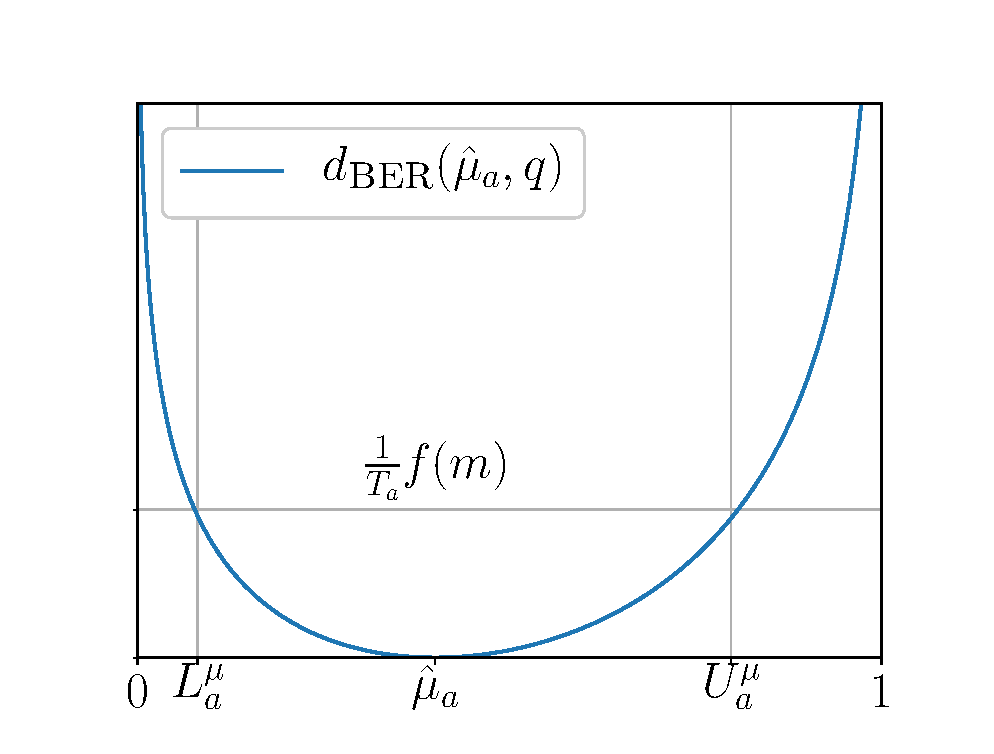
\includegraphics[width=0.6\textwidth]{img/ukl}
	\caption{The Bernoulli Kullback-Leibler divergence $\dber$, and the corresponding upper and lower confidence bounds $U^{\mu}_a$ and $L^{\mu}_a$ for the empirical average $\hat{\mu_a}$. Lower values of $f(m)$ give tighter confidence bounds that hold with lower probabilities.}
	\label{fig:ukl}
\end{figure}

$U^{\mu}_a(m)$ and $L^{\mu}_a(m)$ can be efficiently computed using Newton iterations, as for any $p\in[0, 1]$ the function $q \rightarrow \dber(p,q)$ is strictly convex and increasing (resp. decreasing) on the interval [p, 1] (resp. [0, p]).

Moreover, we use the constant function $f_2: m \rightarrow 2 \log M + 2 \log\log M$. This choice is justified in the end of section \ref{sec:regret-proof}. Because $f_2$ is lower than $f_4$, the Figure \ref{fig:ukl} shows that the bounds are tighter and hence less conservative than that of \OLOP, which should increase the performance, provided that their associated probability of violation does not invalidate the regret bound of \OLOP.


\begin{remark}[Upper bounds sharpening]
	\label{rmk:sharpen}
	\begin{leftbar}[remarkbar]
	The introduction of the B-values $B_a(m)$ was made necessary in \OLOP by the use of Chernoff-Hoeffding confidence bounds which are not guaranteed to belong to [0, 1]. On the contrary, we have in \KLOLOP that $U^\mu_a(m) \in I = [0,1]$ by construction. By Lemma \ref{lemma:seq_values}, the upper bounds sharpening step in line \ref{alg:b_values_compute} of Algorithm \ref{algo:kl-olop} is now superfluous as we trivially have $B_a(m) = U_a(m)$ for all $a\in A^L$.
	\end{leftbar}
\end{remark}

\subsection{Sample complexity}
\label{sec:sample-complexity}

We say that $u_n = \tilde{O}(v_n)$ if there exist $\alpha, \beta >0$ such that $u_n \leq \alpha \log(v_n)^\beta v_n$.
Let us denote the proportion of near-optimal nodes $\kappa_2$ as:


\begin{equation*}
\label{eq:kappa}
\kappa_2 \eqdef \limsup_{h\rightarrow\infty}{\left|\left\{a\in a^H:V(a) \geq V - 2\frac{\gamma^{h+1}}{1-\gamma}\right\}\right|^{1/h}}
\end{equation*}

\begin{theorem}[Sample complexity]
	\label{thm:regret}
	\begin{leftbar}[theorembar]
	We show that \KLOLOP enjoys the same asymptotic regret bounds as \OLOP. More precisely, for any $\kappa' > \kappa_2$, \KLOLOP satisfies:
	
	
	\begin{equation*}
	\expectedvalue r_n = \begin{cases}
	\tilde{0}\left(n^{-\frac{\log 1/\gamma}{\log \kappa'}}\right), & \text{if}\ \gamma\sqrt{\kappa'} > 1 \\
	\tilde{0}\left(n^{-\frac{1}{2}}\right), & \text{if}\ \gamma\sqrt{\kappa'} \leq 1
	\end{cases}
	\end{equation*}
	\end{leftbar}
\end{theorem}

\subsection{Time and memory complexity}
\label{sec:time-complexity}

After having considered the sample efficiency of \OLOP and \KLOLOP, we now turn to study their time and memory complexities. We will only mention the case of \KLOLOP for ease of presentation, but all results easily extend to \OLOP.

The Algorithm \ref{algo:kl-olop} requires, at each episode, to compute and store in memory of the reward upper-bounds and U-values of all nodes in the tree $\Tau = \sum_{h=0}^L A^h$.
Hence, its time and memory complexities are 
\begin{equation}
C(\KLOLOP) = O(M|\Tau|) = O(MK^L).
\end{equation}

The curse of dimensionality brought by the branching factor $K$ and horizon $L$ makes it intractable in practice to actually run \KLOLOP in its original form even for small problems. However, most of this computation and memory usage is wasted, as with reasonable sample budgets $n$ the vast majority of the tree $\Tau$ will not be actually explored and hence does not hold any valuable information.

We propose in Algorithm \ref{algo:lazy-kl-olop} a lazy version of \KLOLOP which only stores and processes the explored subtree, as shown in Figure \ref{fig:tree}, while preserving the inner workings of the original algorithm.

\begin{figure}[ht]
	\centering
	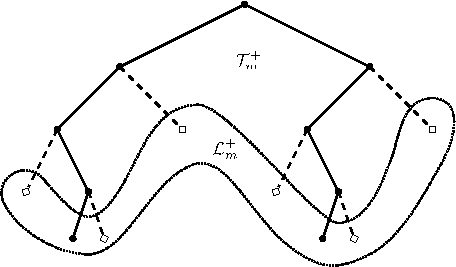
\includegraphics[width=0.6\textwidth]{img/tree_svg-tex}
	\caption{A representation of the tree $\Tau_m^+$, with $K = 2$ actions and after episode $m = 2$, when two sequences have been sampled. They are represented with solid lines and dots \textbullet, and they constitute the explored subtree $\Tau_m$. When extending $\Tau_m$ with the missing children of each node, represented with dashed lines and diamonds $\diamond$, we obtain the full extended subtree $\Tau_m^+$. The set of its leaves is denoted $\LL_m^+$ and shown as a dotted set.}
	\label{fig:tree}
\end{figure}

\begin{algorithm}[tp]
	\DontPrintSemicolon
	Let $M$ be the largest integer such that $M \log M/(2 \log 1/\gamma) \leq n$\;
	Let $L = \log M / (2 \log 1/\gamma)$\;
	Let $\Tau_0^+ = \LL_0^+ = \{\emptyset\}$\;
	\For{each episode $m = 1, \cdots, M$}{
		Compute $U_a(m-1)$ from \eqref{eq:Ua} for all $a\in\Tau_{m-1}^+$\;
		Compute $B_a(m-1)$ from \eqref{eq:Ba} for all $a\in \LL_{m-1}^+$\;
		Sample a sequence with highest B-value: $a \in \argmax_{a\in \LL_{m-1}^+} B_a(m-1)$\;
		Choose an arbitrary continuation $a^m \in aA^{L-|a|}$\tcp*{e.g. uniformly}
		Let $\Tau_m^+ = \Tau_{m-1}^+$ and $\LL_m^+ = \LL_{m-1}^+$\;
		\For{$t=1, \cdots, L$}{
			\If{$a^m_{1:t} \not \in \Tau_{m}^+$}{
				Add $a^m_{1:t-1}A$ to $\Tau_{m}^+$ and $\LL_{m}^+$\;
				Remove $a^m_{1:t-1}$ from $\LL_{m}^+$
			}
		}
	}
	\Return the most played sequence $a(n) \in \argmax_{a\in \LL_m^+} T_a(M)$
	\caption{Lazy Open Loop Optimistic Planning}
	\label{algo:lazy-kl-olop}
\end{algorithm}

\begin{theorem}[Consistency]
	\label{thm:consistency}
	\begin{leftbar}[theorembar]
	The set of sequences returned by Algorithm \ref{algo:lazy-kl-olop} is the same as the one returned by Algorithm \ref{algo:kl-olop}.
	In particular, Algorithm \ref{algo:lazy-kl-olop} enjoys the same regret bounds as in Theorem \ref{thm:regret}.
	\end{leftbar}
\end{theorem}

\begin{proposition}[Time and memory complexity]
	\begin{leftbar}[propositionbar]
	Algorithm \ref{algo:lazy-kl-olop} has time and memory complexities of:
	\begin{equation*}
	C(\texttt{Lazy KL-OLOP}) = O(KLM^2)
	\end{equation*}
	
	The corresponding complexity gain compared to the original Algorithm \ref{algo:kl-olop} is: 
	\begin{equation*}
	\frac{C(\texttt{Lazy KL-OLOP})}{C(\KLOLOP)} = \frac{n}{K^{L-1}}
	\end{equation*}
	which highlights that only a subtree corresponding to the sample budget $n$ is processed instead of the search whole tree $\Tau$.
	\end{leftbar}
\end{proposition}
\begin{proof}
	At episode $m = 1, \cdots, M$, we compute and store in memory the reward upper-bounds and U-values of all nodes in the subtree $\Tau_m^+$. Moreover, the tree $\Tau_m^+$ is constructed iteratively by adding K nodes at most L times at each episode from 0 to $m$. Hence, $|\Tau_m^+| = O(mKL)$.
	This yields directly $C(\texttt{Lazy KL-OLOP}) = \sum_{m=1}^M O(mKL) = O(M^2KL)$.
\end{proof}

\subsection{Proof of Theorem \ref{thm:regret}}
\label{sec:regret-proof}


We follow step-by step the pyramidal proof of \citep{Bubeck2010}, and adapt it to the Kullback-Leibler upper confidence bound. The adjustments resulting from the change of confidence bounds are \diff{highlighted}. The proofs of lemmas which are not significantly altered are listed in the Supplementary Material. 

We start by recalling their notations.
Let $1 \leq H \leq L$ and $a^* \in A^L$ such that $V(a^*) = V$.
Considering sequences of actions of length $1 \leq h \leq H$, we define the subset $\mathcal{I}_h$ of near-optimal sequences and the subset $\mathcal{J}$ of sub-optimal sequences that were near-optimal at depth $h-1$:
\begin{equation*}
\mathcal{I}_h = \left\{a \in A^h: V - V(a) \leq 2\frac{\gamma^{h+1}}{1-\gamma}\right\}, \mathcal{J}_h = \left\{a \in A^h: a_{1:h-1} \in \mathcal{I}_{h-1} \text{ and } a \not\in \mathcal{I}_h\right\}
\end{equation*}

By convention, $\mathcal{I}_0 = \{\emptyset\}$. From the definition of $\kappa_2$, we have that for any $\kappa'>\kappa_2$, there exists a constant C such that for any $h \geq 1$,
%\begin{equation*}
$|\mathcal{I}_h| \leq C {\kappa'}^h$
%\end{equation*}
Hence, we also have $|\mathcal{J}_h| \leq K|\mathcal{I}_{h-1}| = O({\kappa'}^h)$.

Now, for $1\leq m \leq M$, $a \in A^t$ with $t \leq h$, $h'<h$, we define the set $\mathcal{P}^a_{h,h'}(m)$ of suffixes of $a$ in $\mathcal{J}_h$ that have been played at least a certain number of times:
\begin{equation*}
\mathcal{P}^a_{h,h'}(m) = \left\{ b\in a A^{h-t}\cap \mathcal{J}_h : T_b(m) \geq \diff{2f(m)}(h+1)^2\gamma^{2(h'-h+1)} + 1 \right\}
\end{equation*}

and the random variable:

\begin{equation*}
\tau^a_{h,h'}(m) = \mathbbm{1}\{T_a(m-1) < \diff{2f(m)}(h+1)^2\gamma^{2(h'-h+1)} + 1 \leq T_a(m)\}
\end{equation*}

\begin{lemma}[Regret and sub-optimal pulls]
	\label{lemma:expected-regret}
	\begin{leftbar}[lemmabar]
	The following holds true:
	\begin{equation*}
	r_n \leq \frac{2K \gamma^{H+1}}{1-\gamma} +\frac{3K}{M}\sum_{h=1}^H\sum_{a\in\mathcal{J}_h}\frac{\gamma^h}{1-\gamma}T_a(M)
	\end{equation*}
	\end{leftbar}
\end{lemma}


The rest of the proof is devoted to the analysis of the term $\expectedvalue \sum_{a\in \mathcal{J}_h} T_a(M)$. The next lemma describes under which circumstances a suboptimal sequence of actions in $\mathcal{J}_h$ can be selected.

\begin{lemma}[Conditions for sub-optimal pull]
	\label{lemma:sub-optimal-pull}
	\begin{leftbar}[lemmabar]
	Assume that at step $m+1$ we select a sub-optimal sequence $a^{m+1}$: there exist $0 \leq h \leq L,  a\in \mathcal{J}_h$ such that $a^{m+1} \in aA^*$. Then, it implies that one of the following propositions is true:
	\begin{equation}
	\label{eq:cond-ukl}
	\tag{UCB violation}
	\diff{U_{a^*}(m)} < V,
	\end{equation}
	or
	\begin{equation}
	\tag{LCB violation}
	\label{eq:cond-lkl}
	\sum_{t=1}^h \gamma^t \diff{L^{\mu}_{a_{1:t}}(m)} \geq V(a),
	\end{equation}
	or
	\begin{equation}
	\tag{Large CI}
	\label{eq:cond-dkl}
	\sum_{t=1}^h \gamma^t\diff{\left(U^{\mu}_{a_{1:t}}(m) - L^{\mu}_{a_{1:t}}(m)\right)} > \frac{\gamma^{h+1}}{1-\gamma}
	\end{equation}
	\end{leftbar}
\end{lemma}
\begin{proof}
	As $a^{m+1}_{1:h} = a$ and \diff{because the U-values are monotonically increasing along sequences of actions} (see Remark \ref{rmk:sharpen} and Lemma \ref{lemma:seq_values}), we have $U_a(m) \geq U_{a^{m+1}}(m)$. Moreover, by Algorithm \ref{algo:kl-olop}, we have $a^{m+1} = \argmax_{a \in A^L}  U_a(m)$ and $a^*\in A^L$, so $U_{a^{m+1}}(m) \geq U_{a^*}(m)$ and finally $U_a(m) \geq U_{a^*}(m)$.
	
	Assume that \eqref{eq:cond-ukl} is false, then:
	\begin{equation}
	\label{eq:ukl-verifie}
	\sum_{t=1}^h \gamma^t U^{\mu}_{a_{1:t}}(m) + \frac{\gamma^{h+1}}{1-\gamma} = U_a(m) \geq U_{a^*}(m) \geq V
	\end{equation}
	Assume that \eqref{eq:cond-lkl} is false, then:
	\begin{equation}
	\label{eq:lkl-verifie}
	\sum_{t=1}^h \gamma^t L^{\mu}_{a_{1:t}}(m) < V(a),
	\end{equation}
	By taking the difference \eqref{eq:ukl-verifie} - \eqref{eq:lkl-verifie}, 
	\begin{equation*}
	\sum_{t=1}^h \gamma^t \left(U^{\mu}_{a_{1:t}}(m) - L^{\mu}_{a_{1:t}}(m)\right) + \frac{\gamma^{h+1}}{1-\gamma} > V - V(a)
	\end{equation*}
	But $a \in \mathcal{J}_h$, so $V - V(a) \geq \frac{2\gamma^{h+1}}{1-\gamma}$, which yields \eqref{eq:cond-dkl} and concludes the proof.
\end{proof}

\diff{In the following lemma, for each episode $m$ we bound the probability of \eqref{eq:cond-ukl} or \eqref{eq:cond-lkl} by a desired confidence level $\delta_m$, whose choice we postpone until the end of this proof. For now, we simply assume that we picked a function $f$ that satisfies $f(m)\log (m) e^{-f(m)} = O(\delta_m)$. We also denote $\Delta_M = \sum_{m=1}^{M}\delta_m$.}

\begin{lemma}[Boundary crossing probability]
	\label{lemma:boundary-crossing-prob}
	\begin{leftbar}[lemmabar]
	The following holds true, for any $1 \leq h \leq L$ and $m \leq M$,
	\begin{equation*}
	\probability{\text{\eqref{eq:cond-ukl} or \eqref{eq:cond-lkl} is true}} = \diff{O((L+h)\delta_m)}
	\end{equation*}
	\end{leftbar}
\end{lemma}
\begin{proof}
	Since $V \leq \sum_{t=1}^h \gamma^t \mu(a^*_{1:t}) + \frac{\gamma^{h+1}}{1-\gamma}$, we have,
	\begin{align*}
	\probability{\eqref{eq:cond-ukl}} &=  \probability{U_{a^*}(m) \leq V}\\
	&= \probability{\sum_{t=1}^L \gamma^t U^{\mu}_{a^*_{1:t}}(m) \leq \sum_{t=1}^L \gamma^t \mu(a^*_{1:t})}\\
	&\leq \probability{\exists 1\leq t \leq L : U^{\mu}_{a^*_{1:t}}(m) \leq \mu(a^*_{1:t})} \\
	&\leq \sum_{t=1}^L\probability{U^{\mu}_{a^*_{1:t}}(m) \leq \mu(a^*_{1:t})}
	\end{align*}
	
	\diff{In order to bound this quantity, we reduce the question to the application of a deviation inequality. For all $1\leq t\leq L$, we have on the event $\{U^{\mu}_{a^*_{1:t}}(m) \leq \mu(a^*_{1:t})\}$ that $\hat{\mu}_{a^*_{1:t}}(m) \leq U^{\mu}_{a^*_{1:t}}(m) \leq \mu(a^*_{1:t}) < 1$. Therefore, for all $0 < \delta < 1 - \mu(a^*_{1:t})$, by definition of $U^{\mu}_{a^*_{1:t}}(m)$:}
	
	\begin{equation*}
	\diff{d(\hat{\mu}_{a^*_{1:t}}(m), U^{\mu}_{a^*_{1:t}}(m)+\delta) > \frac{f(m)}{T_{a^*_{1:t}}(m)}}
	\end{equation*}
	
	\diff{As $d$ is continuous on $(0,1)\times[0, 1]$, we have by letting $\delta \rightarrow 0$ that:}
	
	\begin{equation*}
	\diff{d(\hat{\mu}_{a^*_{1:t}}(m), U^{\mu}_{a^*_{1:t}}(m)) \geq \frac{f(m)}{T_{a^*_{1:t}}(m)}}
	\end{equation*}
	
	\diff{Since d is non-decreasing on $[\hat{\mu}_{a^*_{1:t}}(m), \mu(a^*_{1:t})]$,}
	
	\begin{equation*}
	\diff{d(\hat{\mu}_{a^*_{1:t}}(m), \mu(a^*_{1:t})) \geq d(\hat{\mu}_{a^*_{1:t}}(m), U^{\mu}_{a^*_{1:t}}(m)) \geq \frac{f(m)}{T_{a^*_{1:t}}(m)}}
	\end{equation*}
	
	\diff{We have thus shown the following inclusion:}
	
	\begin{equation*}
	\diff{\{U^{\mu}_{a^*_{1:t}}(m) \leq \mu(a^*_{1:t})\} \subseteq \left\{ \mu(a^*_{1:t}) > \hat{\mu}_{a^*_{1:t}}(m) \text{ and } d(\hat{\mu}_{a^*_{1:t}}(m), \mu(a^*_{1:t})) \geq \frac{f(m)}{T_{a^*_{1:t}}(m)} \right\}}
	\end{equation*}
	
	\diff{Decomposing according to the values of $T_{a^*_{1:t}}(m)$ yields:}
	
	\begin{equation*}
	\diff{\{U^{\mu}_{a^*_{1:t}}(m) \leq \mu(a^*_{1:t})\} \subseteq \bigcup_{n=1}^m \left\{ \mu(a^*_{1:t}) > \hat{\mu}_{a^*_{1:t}, n} \text{ and } d(\hat{\mu}_{a^*_{1:t}, n}, \mu(a^*_{1:t})) \geq \frac{f(m)}{n} \right\}}
	\end{equation*}
	
	\diff{We now apply the deviation inequality provided in Lemma 2 of Appendix A in \citep{Cappe2013}: $\forall \epsilon > 1$, provided that $0 < \mu(a^*_{1:t}) < 1$,}
	
	\begin{equation*}
	\diff{\probability{\bigcup_{n=1}^m \left\{ \mu(a^*_{1:t}) > \hat{\mu}_{a^*_{1:t}, n} \text{ and } n \dber(\hat{\mu}_{a^*_{1:t}, n}, \mu(a^*_{1:t})) \geq \epsilon \right\}} \leq e\ceil{\epsilon \log m}e^{-\epsilon}\,.}
	\end{equation*}
	
	\diff{By choosing $\epsilon = f(m)$, it comes}
	\begin{align*}
	\diff{\probability{\eqref{eq:cond-ukl}} \leq \sum_{t=1}^L e\ceil{f(m)\log m}e^{-f(m)} = O(L\delta_m)}
	\end{align*}
	
	The same reasoning gives: $\quad\displaystyle{
		\probability{\eqref{eq:cond-lkl}} = \diff{O(h\delta_m)}}$.
\end{proof}

\begin{lemma}[Confidence interval length and number of plays]
	\label{lemma:ci-length}
	\begin{leftbar}[lemmabar]
	Let $1 \leq h \leq L$, $a\in \mathcal{J}_h$ and $0 \leq h' < h$. Then  \eqref{eq:cond-dkl} is not satisfied if the following propositions are true:
	\begin{equation}
	\label{eq:sampled-enough-h}
	\forall 0\leq t\leq h', T_{a_{1:t}}(m) \geq \diff{2f(m)}(h+1)^2\gamma^{2(t-h-1)}
	\end{equation}
	and
	\begin{equation}
	\label{eq:sampled-enough}
	T_{a}(m) \geq \diff{2f(m)}(h+1)^2\gamma^{2(h'-h-1)}
	\end{equation}
	\end{leftbar}
\end{lemma}
\begin{proof}
	We start by providing an explicit upper-bound for the length of the confidence interval $U^{\mu}_{a_{1:t}} - L^{\mu}_{a_{1:t}}$. \diff{By Pinsker's inequality:}
	
	\begin{equation*}
	\diff{\dber(p, q) > \dquad(p, q)}
	\end{equation*}
	
	\diff{Hence for all $C>0$, }
	\begin{equation*}
	\diff{\dber(p, q) \leq C   \implies 2(q - p)^2 < C  \implies p - \sqrt{C/2} < q < p + \sqrt{C/2}}
	\end{equation*}
	\diff{And thus, for all $b\in A^*$, by definition of $U^{\mu}$ and $L^{\mu}$:}
	\begin{align*}
	\diff{U^{\mu}_{b}(m) - L^{\mu}_{b}(m) \leq \frac{S_b(m)}{T_b(m)} + \sqrt{\frac{f(m)}{2T_b(m)}} -  \left(\frac{S_b(m)}{T_b(m)} - \sqrt{\frac{f(m)}{2T_b(m)}}\right) 
		= \sqrt{\frac{2f(m)}{T_b(m)}}}
	\end{align*}
	
	Now, assume that \eqref{eq:sampled-enough-h} and \eqref{eq:sampled-enough} are true. Then, we clearly have:
	\begin{align*}
	\sum_{t=1}^h \gamma^t\left(U^{\mu}_{a_{1:t}}(m) - L^{\mu}_{a_{1:t}}(m)\right) &\leq \sum_{t=1}^{h'} \gamma^t \sqrt{\frac{2f(m)}{T_{a_{1:t}}(m)}} + \sum_{t=h'+1}^h \gamma^t \sqrt{\frac{2f(m)}{T_{a_{1:t}}(m)}} \\
	&\leq \frac{1}{(h+1)\gamma^{-h-1}} \sum_{t=1}^{h'} 1 + \frac{1}{(h+1)\gamma^{-h-1}} \sum_{t=h'+1}^h \gamma^{t-h'}  \\
	&\leq \frac{\gamma^{h+1}}{h+1} \left( h' + \frac{\gamma}{1-\gamma} \right)\leq \frac{\gamma^{h+1}}{1-\gamma}\,.
	\end{align*}
\end{proof}

\begin{lemma}
	\label{lemma:size_Ph}
	\begin{leftbar}[lemmabar]
	Let $1 \leq h \leq L,  a\in \mathcal{J}_h$ and $0\leq h'<h$. Then $\tau^a_{h,h'}=1$ implies that either equation \eqref{eq:cond-ukl} or \eqref{eq:cond-lkl} is satisfied or the following proposition is true:
	
	
	\begin{equation}
	\label{eq:P-min-size}
	\exists 1\leq t \leq h': |\mathcal{P}_{h,h'}^{a_{1:t}}(m)| < \gamma^{2(t-h')}
	\end{equation}
	\end{leftbar}
\end{lemma}

\begin{lemma}
	\label{lemma:expected-P-size}
    \begin{leftbar}[lemmabar]
	Let $1\leq h\leq L$ and $0 \leq h' < h$. Then the following holds true,
	
	\begin{equation*}
	\expectedvalue |\mathcal{P}^\emptyset_{h,h'}(M)| = \tilde{O}\left(\gamma^{-2h'}\mathbbm{1}_{h'>0}\sum_{t=0}^{h'}(\gamma^2 \kappa')^t + (\kappa')^h\diff{\Delta_M} \right).
	\end{equation*}
	\end{leftbar}
\end{lemma}

\begin{lemma}
	\label{lemma:expected-plays-count}
	\begin{leftbar}[lemmabar]
	Let $1\leq h\leq L$. The following holds true,
	\begin{equation*}
	\expectedvalue \sum_{a\in \mathcal{J}_h} T_a(M) = \tilde{O}\left(\gamma^{-2h} + \diff{(\kappa')^h(1+M\Delta_M+\Delta_M) + (\kappa'\gamma^{-2})^h\Delta_M}\right)
	\end{equation*}
	\end{leftbar}
\end{lemma}

Thus by combining Lemma \ref{lemma:expected-regret} and \ref{lemma:expected-plays-count} we obtain:
\begin{equation*}
\expectedvalue r_n = \tilde{O}\left(\gamma^H + \gamma^{-H}M^{-1} + (\kappa' \gamma)^{H}M^{-1}\diff{(1+M\Delta_M+\Delta_M)} + (\kappa')^H\gamma^{-H}M^{-1}\diff{\Delta_M}\right)
\end{equation*}
Finally,
\begin{itemize}
	\item if $\kappa'\gamma^2 \leq 1$, we take $H = \floor{\log M / (2\log 1/\gamma)}$ to obtain:
	\begin{equation*}
	\expectedvalue r_n = \tilde{O}\left(M^{-\frac{1}{2}} + M^{-\frac{1}{2}} + M^{-\frac{1}{2}}M^{\frac{\log \kappa'}{2\log 1/\gamma}} \diff{\Delta_M}\right)
	\end{equation*}
	For the last term to be of the same order of the others, we need to have $\Delta_M = O(M^{-\frac{\log \kappa'}{2\log 1/\gamma}})$. Since $\kappa'\gamma^2 \leq 1$, we achieve this by taking \diff{$\Delta_M = O(M^{-1})$}.
	\item if $\kappa'\gamma^2 > 1$, we take $H = \floor{\log M / \log \kappa'}$ to obtain:
	\begin{equation*}
	\expectedvalue r_n = \tilde{O}\left(M^{\frac{\log \gamma}{\log \kappa'}} + M^{\frac{\log \gamma}{\log \kappa'}}\diff{(1+M\Delta_M+\Delta_M)} + M^{\frac{\log 1/\gamma}{\log \kappa'}}\diff{\Delta_M}\right)
	\end{equation*}
	Since $\kappa'\gamma^2 > 1$, the dominant term in this sum is $M^{\frac{\log \gamma}{\log \kappa'}}M\Delta_M$. Again, taking \diff{$\Delta_M = O(M^{-1})$} yields the claimed bounds.
\end{itemize}
Thus, the claimed bounds are obtained in both cases as long as we can impose $\Delta_M = O(M^{-1})$, that is, find a sequence $(\delta_m)_{1\leq m\leq M}$ and a function $f$ verifying:
\begin{equation}
\sum_{m=1}^M \delta_m = O(M^{-1})\quad \text{and}\quad f(m)\log (m) e^{-f(m)} = O(\delta_m)
\end{equation}

By choosing \diff{$\delta_m = M^{-2}$ and $f(m) = 2 \log M + 2 \log\log M$}, the corresponding \KLOLOP algorithm does achieve the regret bound claimed in Theorem \ref{thm:regret}.


\subsection{Experiments and Conclusion}
\label{sec:planning-experiments}

We have performed some numerical experiments to evaluate and compare the following planning algorithms\footnote[1]{The source code is available at \url{https://eleurent.github.io/kl-olop/}}:
\begin{itemize}
	\item \texttt{Random}: returns a random action, we use it as a minimal performance baseline.
	\item \OPD: the \emph{Optimistic Planning for Deterministic systems} from \citep{Hren2008}, used as a baseline of optimal performance. This planner is only suited for deterministic environments, and exploits this property to obtain faster rates. However, it is expected to fail in stochastic environments.
	\item \OLOP: as described in section \ref{sec:kl-olop-olop}.\footnote[2]{Note that we use the lazy version of $\OLOP$ and $\KLOLOP$ presented in Section \ref{sec:time-complexity}, otherwise the exponential running-time would have been prohibitive.}
	\item \KLOLOP: as described in section \ref{sec:kl-olop-kl-olop}.\footnotemark[2]
	\item \texttt{KL-OLOP}(1): an aggressive version of \KLOLOP where we used $f_1(m) = \log M$ instead of $f_2(m)$. This threshold function makes the upper bounds even tighter, at the cost of an increased probability of violation. Hence, we expect this solution to be more efficient in close-to-deterministic environments. However, since we have no theoretical guarantee concerning its regret as we do with $\KLOLOP$, it might not be conservative enough and converge too early to a suboptimal sequence, especially in highly stochastic environments.
\end{itemize}

They are evaluated on the following tasks, using a discount factor of $\gamma=0.8$:
\begin{itemize}
	\item A \href{https://github.com/eleurent/highway-env/}{highway driving} environment \citep{highway-env}: a vehicle is driving on a road randomly populated with other slower drivers, and must make their way as fast as possible while avoiding collisions by choosing on the the following actions: \texttt{change-lane-left}, \texttt{change-lane-right}, \texttt{no-op}, \texttt{faster}, \texttt{slower}.
	\item A \href{https://github.com/maximecb/gym-minigrid}{gridworld} environment \citep{gym_minigrid}: the agent navigates in a randomly-generated gridworld composed of either empty cells, terminal lava cells, and goal cells where a reward of $1$ is collected at the first visit.
	\item A stochastic version of the gridworld environment with noisy rewards, where the noise is modelled as a Bernoulli distribution with a 15\% probability of error, i.e. receiving a reward of 1 in an empty cell or 0 in a goal cell.
\end{itemize}

\begin{figure}[pth]
	\centering
	\begin{subfigure}[b]{0.8\linewidth}
		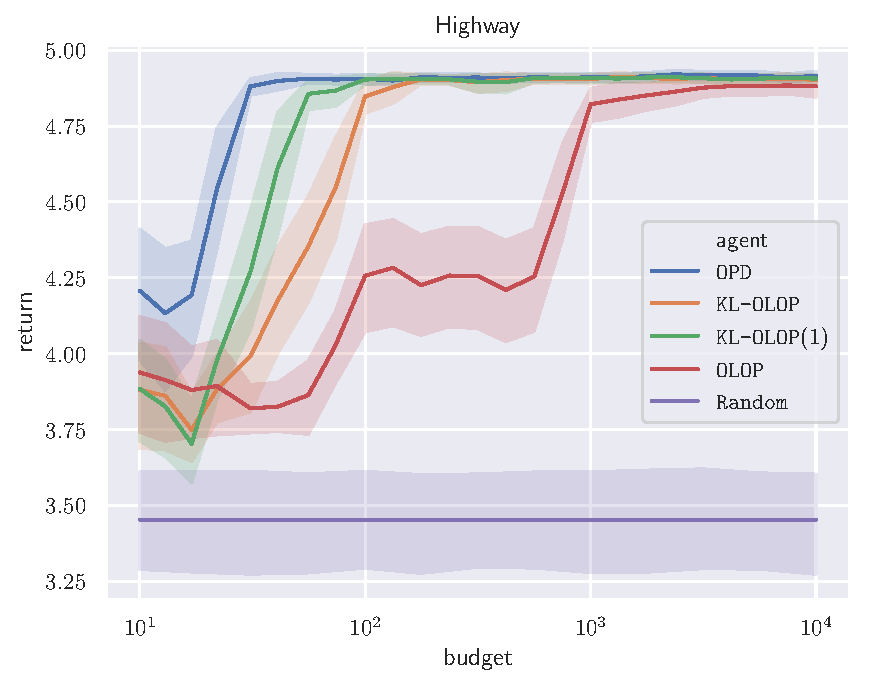
\includegraphics[width=\textwidth]{img/hw_return_svg-tex}
		\caption{Highway}
		\label{sub:highway}
	\end{subfigure}
	\newline
	\begin{subfigure}[b]{0.49\linewidth}
		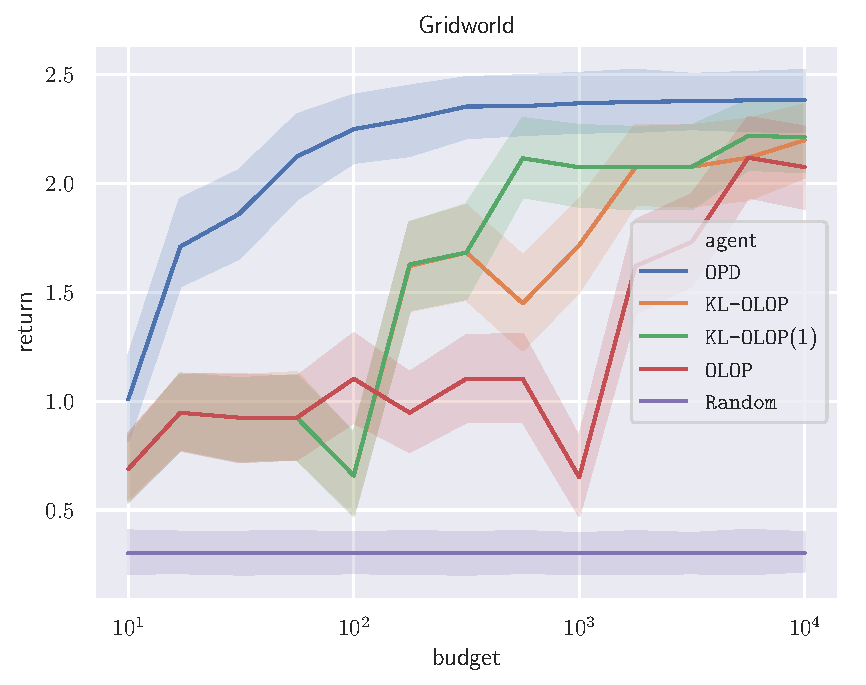
\includegraphics[width=\textwidth]{img/gw_return_svg-tex}
		\caption{Gridworld}
		\label{sub:gridworld}
	\end{subfigure}
	\begin{subfigure}[b]{0.49\linewidth}
		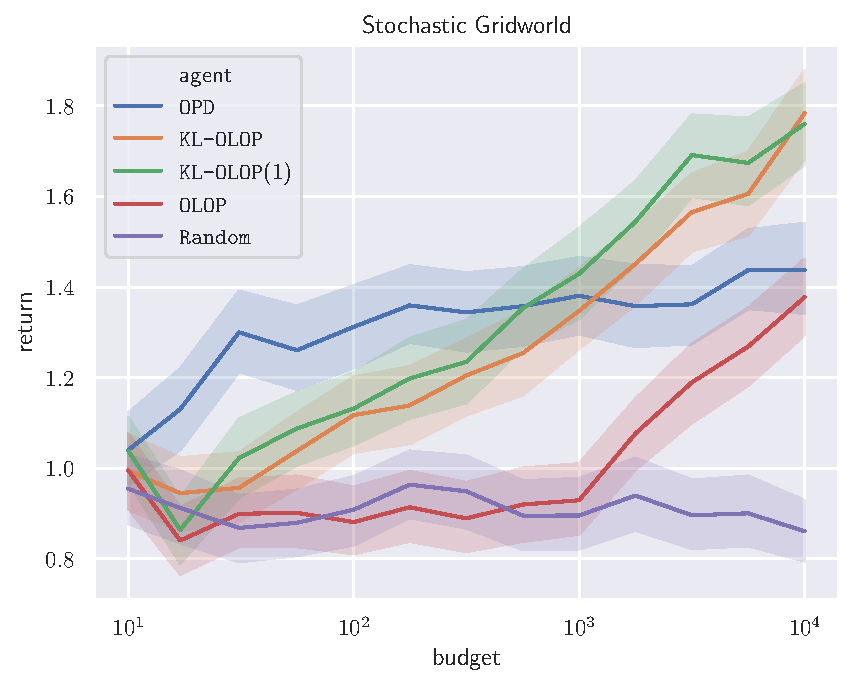
\includegraphics[width=\textwidth]{img/gw_stoch_return_svg-tex}
		\caption{Stochastic Gridworld}
		\label{sub:gridworld_stoch}
	\end{subfigure}
	\caption{Numerical experiments: for each environment-agent configuration, we compute the average return over 100 runs –- along with its 95\% confidence interval –- with respect to the available budget $n$.}
	\label{fig:experiments}
\end{figure}

\begin{figure}[pth]
	\centering
	
	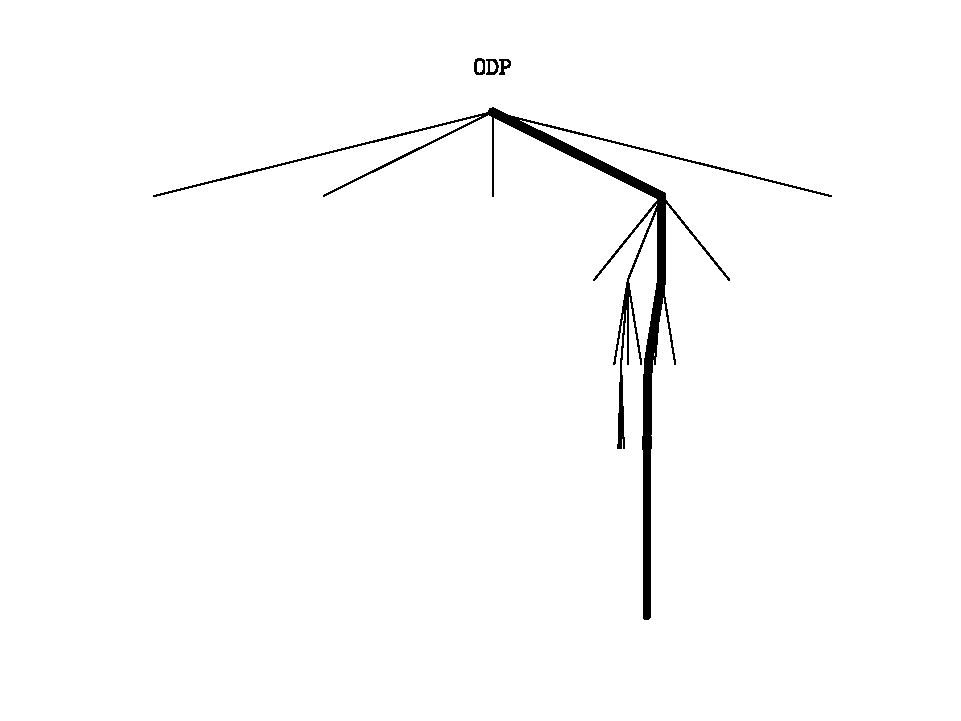
\includegraphics[width=0.6\textwidth]{img/tree_OPD_svg-tex} 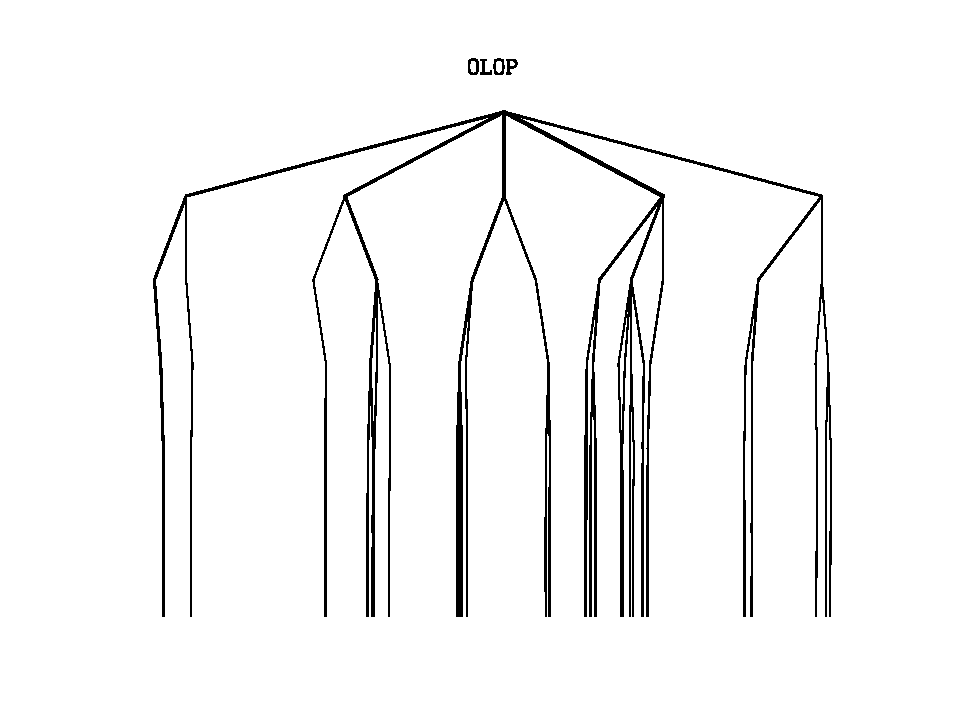
\includegraphics[width=0.6\textwidth]{img/tree_OLOP_svg-tex}
	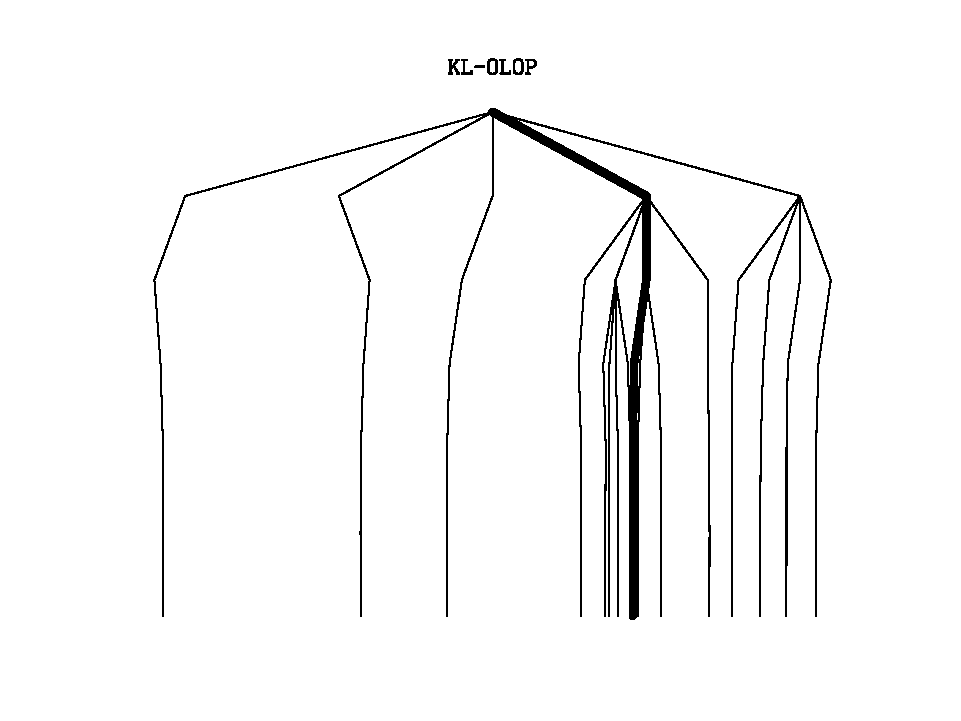
\includegraphics[width=0.6\textwidth]{img/tree_KL-OLOP_svg-tex}
	
	\caption{The look-ahead trees (down to depth 6) expanded by the planning algorithms from the same initial state in the highway environment with the same budget $n=10^3$. The width of edges represents the nodes visit count $T_a(M)$.}
	\label{fig:trees}
\end{figure}

The results of our experiments are shown in Figure \ref{fig:experiments}. The \OPD algorithm converges very quickly to the optimal return in the two first environments, shown in Figure \ref{sub:highway} and Figure \ref{sub:gridworld}, because it exploits their deterministic nature: it needs neither to estimate the rewards through upper-confidence bounds nor to sample whole sequences all the way from the root when expanding a leaf, which provides a significant speedup. It can be seen as an oracle allowing to measure the conservativeness of stochastic planning algorithms. And indeed, even before introducing stochasticity, we can see that \OLOP performs quite badly on the two environments, only managing to solve them with a budget in the order of $10^{3.5}$. In stark contrast, \KLOLOP makes a much better use of its samples and reaches the same performance an order of magnitude faster. This is illustrated by the expanded trees shown in Figure \ref{fig:trees}: \OPD exploits the deterministic setting and produces a sparse tree densely concentrated around the optimal trajectory. Conversely, the tree developed by \OLOP is evenly balanced, which suggests that \OLOP behaves as uniform planning as hypothesised in Section \ref{sec:kl-olop-behaviour}. \KLOLOP is more efficient and expands a highly unbalanced tree, exploring the same regions as \OPD. Furthermore, in the stochastic gridworld environment shown in Figure \ref{sub:gridworld_stoch}, we observe that the deterministic \OPD planner's performance saturates as it settles to suboptimal trajectories, as expected. Conversely, the stochastic planners all find better-performing open-loop policies, which justifies the need for this framework. Again, \KLOLOP converges an order of magnitude faster than \OLOP. Finally, \texttt{KL-OLOP}(1) enjoys good performance overall and displays the most satisfying trade-off between aggressiveness in deterministic environments and conservativeness in stochastic environments; hence we recommend this tuning for practical use.

\subsection{Conclusion}

We introduced an enhanced version of the \OLOP algorithm for open-loop online planning, whose design was motivated by an investigation of the over-conservative search behaviours of \OLOP. We analysed its sample complexity and showed that the original regret bounds are preserved, while its empirical performances are increased by an order of magnitude in several numerical experiments. Finally, we proposed an efficient implementation that benefits from a substantial speedup, facilitating its use for real-time planning applications.


\section{On a closed-loop algorithm}

We briefly mention an extension of \KLOLOP to closed-loop policies, in the setting where the transitions have a finite support of size $B < \infty$. The algorithm, named \MDPGapE, was developed as part of a collaboration \citep{jonsson2020planning} and analysed in the fixed-confidence setting.

It relies on estimating confidence sets $\cC_t$ on the probability vector $p(\cdot|s,a)$
$$\cC_t(s,a) \eqdef \left\{p\in \Sigma_S :  \KL\!\big(\hp_t(\cdot|s,a),p\big) \leq \frac {\beta^p(n_t(s,a), n)} {n_t(s,a)}\right\},$$

and forming recursive upper and lower confidence bounds in the form
\begin{align*}
U_{h}(s) &= \max_{a\in A} \left[u_t(s,a) + \gamma \max_{q \in \cC_t(s,a)} \sum_{s'} q(s'|s,a) U_{h+1}(s')\right], \\
L_{h}(s) &= \max_{a\in A} \left[\ell_t(s,a) + \gamma \min_{q \in \cC_t(s,a)} \sum_{s'} q(s'|s,a)L_{h+1}(s')\right].
\end{align*}

\section{Graph-based optimistic planning}
\label{sec:gbopd}

We start by considering the simple setting of MDPs with deterministic dynamics and rewards, and will denote $r(s,a)$ and $P(s,a)$ the unique reward $r$ and next state $s'$ sampled from $P\left(r,s'|s,a\right)$, respectively.
Let us give some background on the interplay of data structures and optimistic planning algorithms.

\subsection{Data structures}

In this work, we compare two data structures for planning in an MDP: tree and (directed) graph, represented in \Cref{fig:structures}. In order to distinguish them, we use Roman symbols when referring to trees, e.g. $T, U, L, B$ and calligraphic symbols when referring to graphs, e.g. $\cG, \cU, \cL, \cB$. In both structures, we say that a node is \emph{internal} if it has outgoing edges, and \emph{external} else.

\begin{figure}[tp]
	\centering
	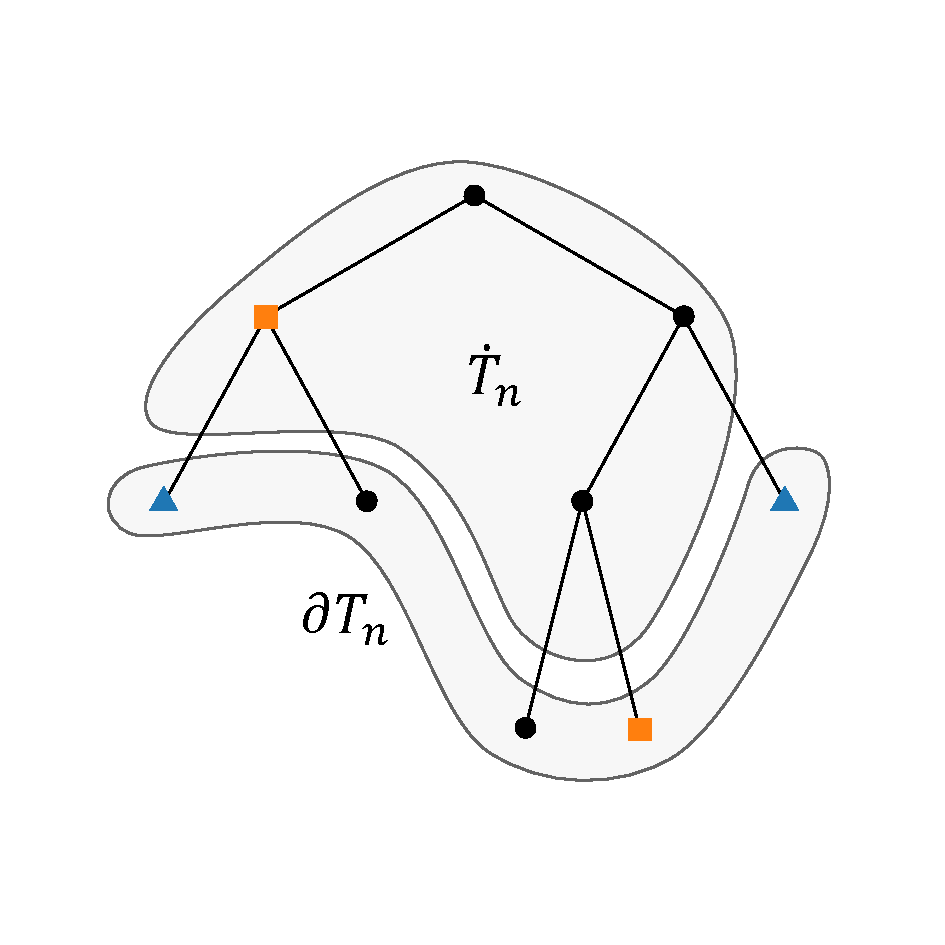
\includegraphics[trim={1.8cm 2.2cm 1.9cm 2.7cm}, clip,width=0.46\linewidth]{img/gbop/tree_1}
	\hfill
	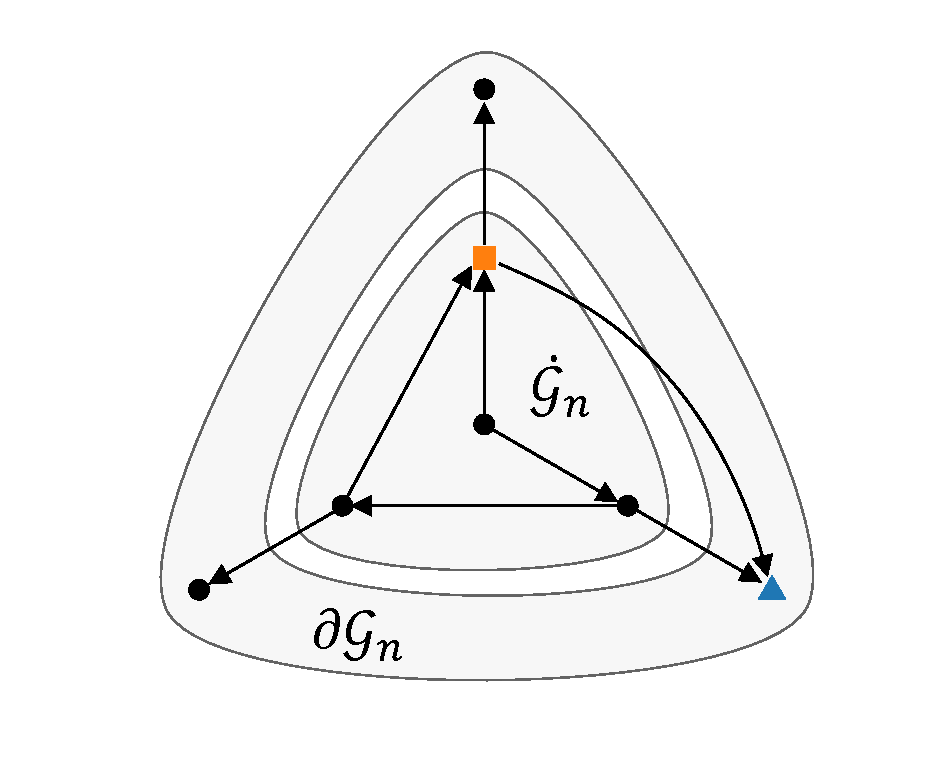
\includegraphics[trim={1.8cm 1.2cm 1.9cm 0.8cm}, clip,width=0.46\linewidth]{img/gbop/graph_1}
	\caption{Illustration of the tree $\Tau_n$ (left) and the graph $\cG_n$ (right) built with the same observed transitions. In the tree, two nodes with the same colour and shape (not black nor round) lead to the same state.}
	\label{fig:structures}
\end{figure}

In a tree, a node of depth $h$ represents a sequence of actions $a\in A^h$. The \textit{root} of the tree corresponds to the empty action sequence, and hence to the initial state $s_0\in S$. At iteration $n$, we denote the current tree as $\Tau_n$. Borrowing notations from topology, we denote its set of internal nodes as $\inte{\Tau}_n$ and its set of external nodes (the leaves) as $\ext{\Tau}_n$. Note that since the MDP is deterministic, a sequence of action $a$ is associated with its final state denoted $s(a)$, but this association is not one-to-one: several sequences of action can lead to the same state, which will be represented several times in the tree.

In a graph, the nodes represent states $s\in S$, and the edges represent transitions between states. The \textit{source} of the graph corresponds to the initial state $s_0$. At iteration $n$, we denote the current graph as $\cG_n$, its set of internal nodes as $\inte{\cG}_n$ and its set of \textit{sinks} as $\ext{\cG}_n$.

Both structures are built iteratively from a single starting node, by selecting an external node (leaf or sink) to expand. The \emph{expansion} of a node $a$ or $s$ refers to calling the generative model to sample the reward $r$ and next state $s'$ for each action $a\in A$, and adding child nodes to the data structure. In a tree, the expansion of a node $a\in A^h$ always lead to the creation of new leaves that represent the suffix sequence of action $ab\in A^{h+1},\, b\in A$. The maximum depth of an expanded node in $T_n$ is denoted $d_n$. In contrast, in a graph the next state $s'$ reached from $s,a$ might already be present in $\cG_n$, in which case we add the edge between $s$ and $s'$ without creating a new node.
These data structures can be used to store information about the MDP, such as the transitions and rewards $r(s, a)$, or other informations useful for planning.


\subsection{Optimistic planning}

A planning algorithm is typically composed of two main rules:
\begin{enumerate*}[label=(\roman*)]
	\item A \emph{sampling rule}, that selects promising transitions to simulate at each iteration $n$;
	\item A \emph{recommendation rule}, that recommends a good first action $a_n$ 	to take (in $s_0$).
\end{enumerate*}
%The pseudo-code of generic planning algorithm is provided in \Cref{alg:generic}.
%\begin{algorithm}
%	\caption{A generic planning algorithm}
%	\label{alg:generic}
%	\DontPrintSemicolon
%	\For{each iteration $n$}{
%		Select the node $b_n$ (or $\hat{s_n}$) to expand according to the \textbf{sampling rule}.\;
%		\For(\Comment*[f]{Node expansion}){action $a\in A$}{
%			Simulate the transition $r, s' \sim P\left(r, s' \condbar s, a\right)$ from the generative model.\;
%			Insert the observed transition to the data structure accordingly.
%		}
%	}
%	\Return the recommended action $a_{n}$ according to the \textbf{recommendation rule}.\;
%\end{algorithm}
These rules can be chosen with the goal of minimising the simple regret $r_n$.
A popular approach is to follow the principle of \emph{Optimism in the Face of Uncertainty} (OFU) \citep[see][]{Munos14}, which consists in exploring the option that maximises an upper-bound of the true objective. In the context of planning, it has been applied by forming bounds on the value function $V$.

\begin{definition}[Value bounds]
	\begin{leftbar}[defnbar]
	{\textbf{On trees.}} We denote by $L:\Tau_n \rightarrow \Real$ and  $U:\Tau_n \rightarrow \Real$ a lower-bound and upper-bound for the state value $V$ defined on the tree $\Tau_n$, such that
	\begin{equation*}
	\forall a\in\Tau_n, \qquad L(a) \leq V(s(a)) \leq U(a).
	\end{equation*}
	
	{\textbf{On graphs.}} Likewise, we denote by $\cL:\cG_n \rightarrow \Real$ and  $\cU:\cG_n \rightarrow \Real$ a lower-bound and upper-bound for the state value $V$ defined on the graph $\cG_n$, such that
	\begin{equation*}
	\forall s\in\cG_n, \qquad \cL(s) \leq V(s) \leq \cU(s).
	\end{equation*}
	\end{leftbar}
\end{definition}

Following the OFU principle, at iteration $n$ we must leverage available information to design an upper-bound $U_n$ (or $\cU_n$) on $V$ as tight as possible. Then, in order to select a promising external node to expand, the sampling rule starts from the root (or source) and follows the optimistic strategy of always selecting the action which maximises $U_n$ (or $\cU_n$), until reaching an optimistic leaf (or sink) to expand. This strategy was used in \citep[e.g.][]{Kocsis06UCT, Hren2008optimistic, Bubeck2010open, Busoniu2012optimistic}.

For instance, since we assume that the rewards are bounded in [0, 1], trivial bounds on $V(s)$ are
$0 \leq V(s) \leq V_{\max} \eqdef {1}/({1-\gamma})$. But these trivial bounds are the same for every node, which makes them non-informative, and do not make use of the observed information. However, they can be used as a valid starting point. Every observed transition stored can then be used to tightened these bounds, by resorting to the Bellman optimality operator.

\begin{definition}[Bellman optimality operator]
	\begin{leftbar}[defnbar]
	\label{def:bellman}
	{\textbf{On trees.}} We define the Bellman optimality operator $B_n$ on the tree $\Tau_n$ as:
	\begin{equation}
	\label{eq:bellman-tree}
	B_n(f)(a) \eqdef \begin{cases}
	\max_{b\in A} r(s(a), b) + \gamma f({ab})
	& \text{if $a\in\inte{\Tau}_n$.} \\
	f(a) & \text{if $a\in\ext{\Tau}_n$;}
	\end{cases}
	\end{equation}
	
	{\textbf{On graphs.}} Likewise, we define the Bellman optimality operator $\cB_n$ on the graph $\cG_n$ as:
	\begin{equation}
	\label{eq:bellman-graph}
	\cB_n(f)(s) \eqdef \begin{cases}
	\max_{b\in A} r(s, b) + \gamma f(P(s,b))
	& \text{if $s\in\inte{\cG}_n$.} \\
	f(s) & \text{if $s\in\ext{\cG}_n$;}
	\end{cases}
	\end{equation}
	The updates of both Bellman operators are depicted in \Cref{fig:bellman}.
	\end{leftbar}
\end{definition}

\begin{remark}
	\begin{leftbar}[remarkbar]
	For ease of notation, we will sometimes drop the $n$ index on $B$ and $\cB$ when it is non-ambiguous.
	\end{leftbar}
\end{remark}


\begin{figure}[tp]
	\centering
	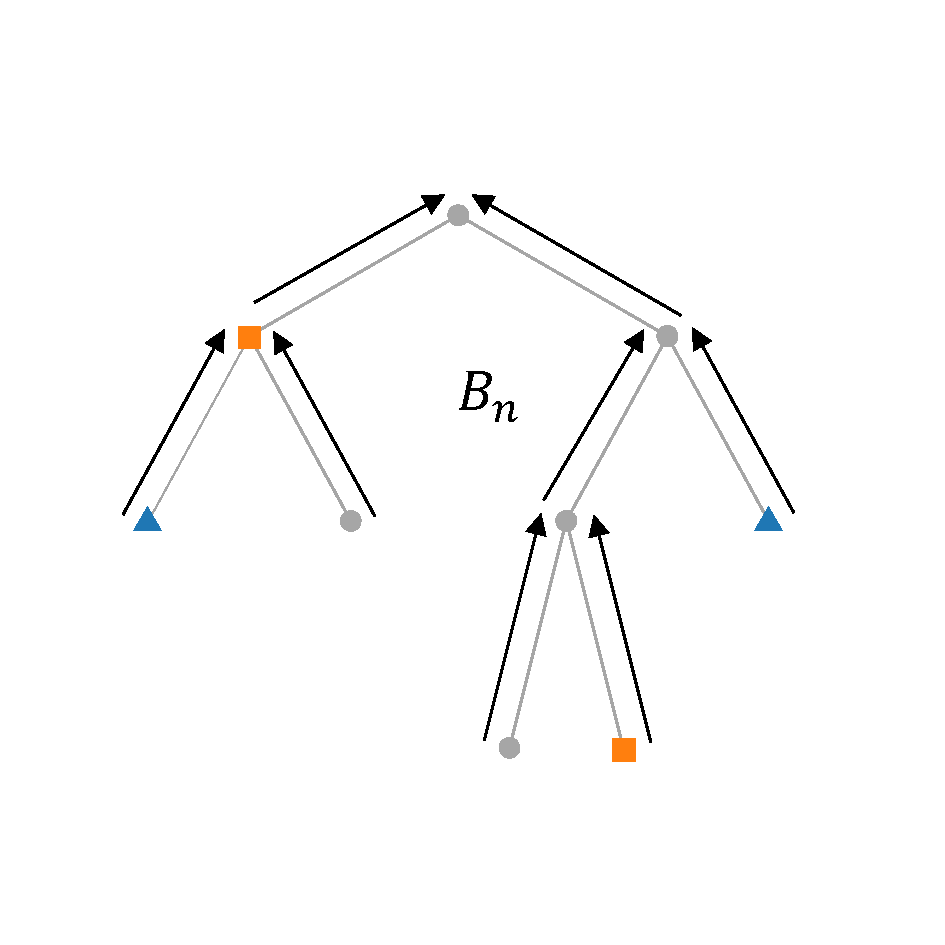
\includegraphics[trim={2.0cm 2.9cm 2.5cm 3.1cm}, clip,width=0.44\linewidth]{img/gbop/tree_2}
	\hfill
	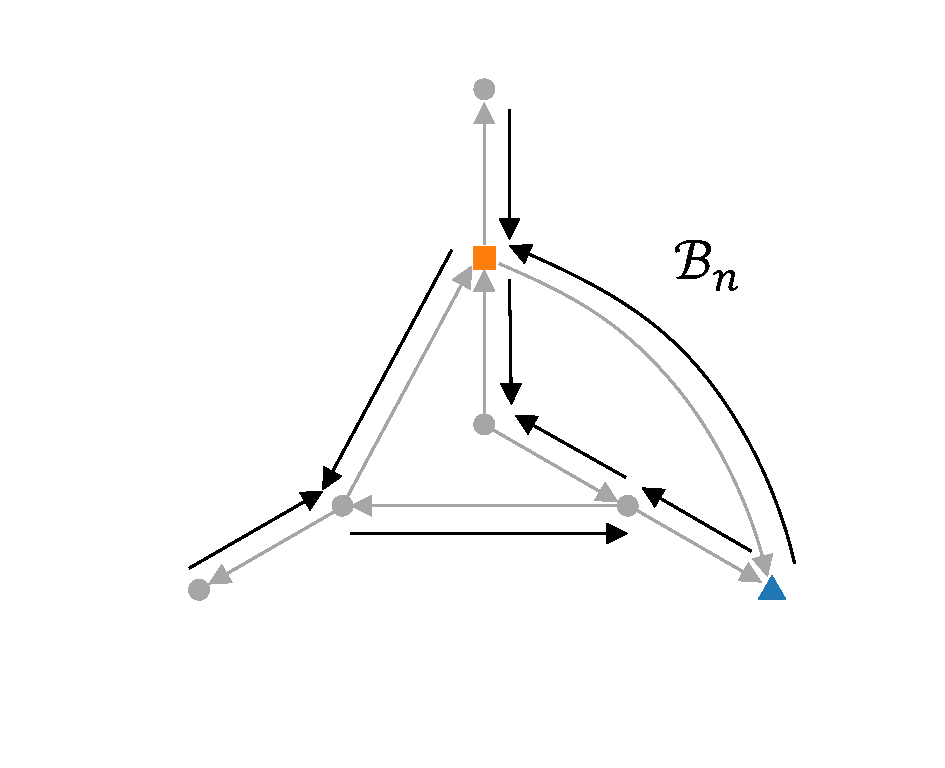
\includegraphics[trim={2.7cm 2.7cm 2.7cm 1.1cm}, clip,width=0.44\linewidth]{img/gbop/graph_2}
	\caption{Illustration of the Bellman backup operators $B$ (left) and $\cB$ (right). Notice that $B_n$ only propagates information upward in the tree.}
	\label{fig:bellman}
\end{figure}

\citet{Hren2008optimistic} used this Bellman operator $B_n$ in their \texttt{OPD} algorithm to define a pair of bounds $(L_n,\, U_n)$ at each iteration $n$. They use trivial bounds at the leaves, and backup these estimates up to the root by iteratively applying $B_n$. We can show that, under a \textit{monotonicity} condition (satisfied by the trivial bounds $0$ and $V_{max}$), applying $B_n$ can only tighten a bound and converges in a finite time.

\begin{definition}[Monotonicity]
	\begin{leftbar}[defnbar]
	A pair of bounds ($L$, $U$) or $(\cL, \cU)$ is \emph{monotonic} if they are respectively non-decreasing and non-increasing along transitions:
	\begin{align*}
	\forall a\in{\Tau}_n, \quad & L(a) \leq B_n(L)(a), & U(a) & \geq B_n(U)(a)\\
	\forall (s)\in\inte{\cG}_n, \quad &\; \cL(s) \leq \cB_n(\cL)(s),&   \cU(s) & \geq \cB_n(\cU)(s)
	\end{align*}
	\end{leftbar}
\end{definition}

\begin{lemma}[Properties of $B_n$]
	\begin{leftbar}[lemmabar]
	\label{lem:properties-b-tree}
	\begin{enumerate}[label=(\roman*)]
		\item $B_n$ preserves monotonicity and tightens monotonic bounds: $$
		\text{if } L\leq V\leq U \text{, then } L \leq B_n(L) \leq V \leq B_n(U) \leq U;
		$$
		\item $(B_n^k)_k$ converges in a finite time $d_n$, where $d_n$ is the depth of $T_n$. 
	\end{enumerate}
	\end{leftbar}
\end{lemma}
This enables \citet{Hren2008optimistic} to define\footnote{We use an iteration of operators while a recursive definition was used originally.} non-trivial valid bounds on $V$:
\begin{align}
\label{eq:opd-bounds}
L_n \eqdef B_n^{d_n}(0), \qquad U_n \eqdef B_n^{d_n}(V_{\max}),
\end{align}
where $0$ is the null function.
The corresponding \texttt{OPD} algorithm is described in \Cref{alg:opd}. Likewise, we have:
\begin{lemma}[Properties of $\cB_n$]
	\begin{leftbar}[lemmabar]
	\label{lem:properties-b-graph}
	\begin{enumerate}[label=(\roman*)]
		\item $\cB_n$ preserves monotonicity and tightens monotonic bounds: $$
		\text{if } \cL\leq V\leq \cU \text{, then } \cL \leq \cB_n(\cL) \leq V \leq \cB_n(\cU) \leq \cU;
		$$
		\item $\cB$ is a $\gamma$-contraction, and we denote $\cB_n^{\infty} \eqdef \lim_{k\rightarrow \infty} \cB_n^k$.
	\end{enumerate}
	\end{leftbar}
\end{lemma}
which motivates us to propose \Cref{alg:gbop-d}, following the approach of \Cref{alg:opd} adapted to a graph structure.

\begin{algorithm}[th]
	\caption{The \emph{Optimistic Planning of Deterministic Systems} (\OPD) algorithm from \citep{Hren2008optimistic}.}
	\label{alg:opd}
	\DontPrintSemicolon
	\For{each iteration $n$}{
		Compute the bounds $L_n = B_n^{d_n}(0)$ and $U_n = B_n^{d_n}(V_{\max})$.\; 
		
		$b_n$ = $\emptyset$\;
		\While{$b_n\in\inte{\Tau}_n$}{
			$b_n\gets \displaystyle\argmax_{a'\in b_n A} r(a') + \gamma U(a')$ \Comment*[r]{Optimistic sampling rule}
		}
		\For(\Comment*[f]{Node expansion}){action $a\in A$}{
			Simulate $r, s' \sim P\left(r, s' \condbar s(b_n), a\right)$.\;
			Add a new leaf $b_n a$ to $\Tau_{n+1}$, with associated reward $r$.
		}
	}
	\Return $\displaystyle\argmax_{a\in A} r(s, a) + \gamma L_n(a)$. \Comment*[r]{Conservative recommendation rule}\;
\end{algorithm}

\begin{algorithm}[th]
	\caption{Our proposed \emph{Graph-Based Optimistic Planning for Deterministic systems} (\GBOPD) algorithm.}
	\label{alg:gbop-d}
	\DontPrintSemicolon
	\For{each iteration $n$}{
		\nl Compute the bounds $\cL_n = \cB_n^{\infty}(0)$ and $\cU_n = \cB_n^\infty(V_{\max})$.\; 
		
		$\hat{s}_n$ = $s_0$\;
		\nl \While{$s_n\in\inte{\cG}_n$}{
			$s_n\gets \displaystyle\argmax_{s'} r(s_n, a) + \gamma \cU_n(s')$ \Comment*[r]{Optimistic sampling rule}
		}
		\For(\Comment*[f]{Node expansion}){action $a\in A$}{
			Simulate $r, s' \sim P\left(r, s' \condbar s_n, a\right)$.\;
			Get or create the node $s'$ in $\cG_{n+1}$, and add the transition $(s_n,a) \rightarrow s', r$.
		}
	}
	\Return $\displaystyle\argmax_{a\in A} r(s,a) + \gamma \cL_n(s(a))$. \Comment*[r]{Conservative recommendation rule}
\end{algorithm}

\begin{remark}[Termination and complexity]
	\begin{leftbar}[remarkbar]
	There are two procedures in \GBOPD that may not terminate in finite time when $\cG_n$ contains a loop:
	\begin{enumerate*}[label=(\roman*)]
		\item the computation of $\cB_n^\infty$ (line 1); and
		\item the sampling rule loop (line 2),
	\end{enumerate*}
	In the Supplementary Material, we discuss an approximate implementation where these two procedures are stopped whenever they reach a desired accuracy $\varepsilon$, along with an analysis of the corresponding time complexity and impact on the planning performance.
	\end{leftbar}
\end{remark}

Though both algorithms share a similar design, we claim that using graphs provides substantial theoretical and practical performance improvements, and back up this statement in \Cref{sec:analysis,sec:experiments}.

\subsection{Analysis}
\label{sec:analysis}

Comparing \OPD and \GBOPD directly is difficult since they do not involve the same structure, which implies implicit differences in their behaviours. Studying them under a common framework would make these differences explicit. To leverage the analysis of \OPD by \citet{Hren2008optimistic}, we frame \GBOPD as a tree-based planning algorithm. To account for the distinction between the operators $B$ and $\cB$, we represent $\cB$ as tree backup $B$ applied on an \emph{unrolled} tree $T(\cG_n)$.

\subsubsection{Background on the sample complexity of \OPD}

First, we recall the analysis of \citet{Hren2008optimistic}. We start by introducing some notations.

\begin{definition}[Sequence values]
	\begin{leftbar}[defnbar]
	The value of a finite \textbf{sequence} of actions $a\in A^h$ is:
	\begin{equation*}
	\label{eq:state_value}
	V(a) = R(s_0,a) + \gamma^{h} V(s(a)),
	\end{equation*}
	where $R(s, a) = \sum_{t=0}^{h-1} \gamma^t r_t$ is the return obtained by executing the sequence of actions $a$ starting from the state $s$.
	\end{leftbar}
\end{definition}

This enables to define a measure of the difficulty of a planning problem.

\begin{definition}[Difficulty measure]
	\begin{leftbar}[defnbar]
	We define the near-optimal branching factor $\hlrb{\kappa}$ of an MDP as
	\begin{equation}
	\hlrb{\kappa = \limsup_{h\rightarrow\infty} |\hlrb{\Tau_h^\infty}|^{1/h}} \in [1, K]
	\end{equation}
	where $\Tau^\infty_h = \displaystyle \left\{a\in A^h: V^\star-V(a) \leq \frac{\gamma^h}{1-\gamma}\right\}$ is the set of near-optimal nodes at depth $h$.
	\end{leftbar}
\end{definition}

This problem-dependent measure $\hlrb{\kappa}$ is the branching factor of the subtree $T^\infty=\bigcup_h T_h^\infty$ of near-optimal nodes that can be sampled by \OPD, and acts as an effective branching factor as opposed to the true branching factor $K$. When $\hlrb{\kappa}$ is small, fewer nodes must be explored at a given depth allowing the algorithm to plan deeper for a given budget $n$. Thus, it directly impacts the simple regret that can be achieved by \OPD when run on a given MDP.


\begin{theorem}[Regret bound of \citealt{Hren2008optimistic}]
	\begin{leftbar}[theorembar]
	\label{thm:regret-opd}
	The \Cref{alg:opd} enjoys the following regret bound:
	\begin{align*}
	\quad r_n = \tilde{\cO}\left( n^{-\log \frac{1}{\gamma}/\hlrb{\log\kappa}}\right),
	\end{align*}
	where $f_n = \tilde{\cO}(n^{-\alpha})$ means that for any $\alpha'<\alpha$, $f_n = \cO(n^{-\alpha'}).$
	\end{leftbar}
\end{theorem}

The near-optimal branching factor $\hlrb{\kappa}$ is related \citep{Bubeck2010} to the near-optimality dimension studied in the online optimisation literature \citep[see e.g.][]{Bubeck2009,Munos2011}.
It is typically small in problems where there is one single optimal trajectory, of which any deviation can be quickly dismissed as suboptimal. Conversely, $\kappa$ is large when many sub-optimal trajectories cannot be distinguished easily based on their values, which requires the exploration of a large part of the tree $T$ of branching factor $K$. 


\subsubsection{Motivation for an improved regret bound}

We start by reformulating the sampling rule used for the \texttt{OPD} algorithm. To that end, notice that when some bounds $(L,\,U)$ on the state values $V(s(a))$ are available, they also induce bounds $(\overline{L},\, \overline{U})$ on values $V(a)$ of sequences of actions $a$ of length $h$ defined as:
\begin{equation*}
%\label{eq:sequence_value}
\underbrace{R(s_0,a) + \gamma^{h} L(a)}_{\overline{L}(a)} \leq V(a) \leq \underbrace{R(s_0,a) + \gamma^{h} U(a)}_{\overline{U}(a)}.
\end{equation*}

One can easily see that, since the $(L_n,\,U_n)$ used in the optimistic sampling rule described in \Cref{alg:opd} are invariant by $B_n$ by definition, this rule can be equivalently expressed as:
\begin{equation}
\label{eq:sampling_rule}
b_n \in \argmax_{a\in\ext{\Tau}_n} \overline{U}_n(a).
\end{equation}
Likewise, the conservative recommendation rule returns the first action of:
\begin{equation}
\label{eq:recommendation_rule}
a_n \in \argmax_{a\in\ext{\Tau}_n} \overline{L}_n(a)
\end{equation}


As shown in \Cref{fig:bellman}, in a tree the Bellman operator $B_n$ only propagates the information upward, and the leaves cannot be updated. Thus, $U_n = B_n^{d_n}(V_{\max})$ and $V_{\max}$ coincide on $\ext{\Tau}_n$ which means that the sampling rule of \texttt{OPD} can be summarized as using \eqref{eq:sampling_rule} with the trivial upper-bound $U_n = V_{\max}$.
Likewise, the recommendation rule simply uses \eqref{eq:recommendation_rule} with the trivial lower-bound $L_n = 0$. Thus, \texttt{OPD} amounts to simply using the trivial bound $(0,\, V_{\max})$ on leaf nodes, and does not make use of all the available information in $\Tau_n$ to improve these bounds.

Let us now assume for the moment that we had access to tighter bounds $(L,\,U)$ provided by an oracle: $$0\leq L\leq V\leq U\leq V_{\max}.$$
\vspace*{-0.5cm}
\begin{definition}[A finer difficulty measure]
	\begin{leftbar}[defnbar]
	We define the near-optimal branching factor \emph{according to the bounds $(L,\,U)$} as 
	\begin{equation}
	\hlbb{\kappa(L,U) \eqdef \limsup_{h\rightarrow\infty} \left|\Tau_h^\infty(L,U)\right|^{1/h}}\in(1, K], 
	\end{equation}
	where
	$ \displaystyle
	{\Tau_h^\infty(L,U)}=\left\{a\in A^h: V^\star - V(a)\leq \gamma^{h}(U(a)-L(a))\right\}.
	$
	\end{leftbar}
\end{definition}

\begin{lemma}
	\begin{leftbar}[lemmabar]
	\label{lem:shrink}
	This branching factor shrinks as the bounds $(L,\,U)$ get tighter:
	\[L_2\leq L_1\leq V\leq U_1\leq U_2\implies \kappa(L_1,U_1) \leq \kappa(L_2,U_2).\]
	In particular, $\hlbb{\kappa(L,U)} \leq \hlrb{\kappa}$.
	\end{leftbar}
\end{lemma}

\begin{theorem}
	\begin{leftbar}[theorembar]
	\label{thm:regret-bound-U}
	Let $L \leq V\leq U$ monotonic bounds, then planning with $L$ and $U$ in \eqref{eq:sampling_rule} and \eqref{eq:recommendation_rule} yields the following simple regret bound:
	\begin{equation*}
	r_n = \tilde{\cO}\left(n^{-\log \frac{1}{\gamma}/\hlbb{\log \kappa(L,U)}}\right).
	\end{equation*}
	\end{leftbar}
\end{theorem}


This theorem states that we can potentially improve the performance of the planning algorithm if we manage to find bounds $(L,\, U)$ that are tighter than the trivial ones at the leaves $\ext{\Tau_n}$, which may be possible if we have already seen the states corresponding to this leaves, but it does not explain how to obtain such bounds. In the next subsection, we describe a method to build a sequence of increasingly tight bounds $(L_n,\, U_n)$, at each planning iteration $n$. The corresponding regret bound, our main result, is stated in \Cref{thm:regret-gbop}.


\subsubsection{Unrolling the tree to tighten the bounds}
\label{sec:unrolling}

In order to reproduce the behaviour of \Cref{alg:gbop-d} on a tree structure, we rely on the following observation:  expanding a node $s$ in $\cG_n$ simultaneously expands all the paths leading to this node.
To account for this observation in the analysis, we will consider an \emph{unrolling} operator $T$ that builds a potentially infinite tree $T(\cG_n)$ containing every sequence of action that can be traversed in a graph $\cG_n$.

\begin{equation}
T(\cG_n) = \{a\in A^h: s_{t+1} \in \cG_n \text{ with } s_{t+1} = P(s_{t}, a_t)\text{ for } 0 \leq t < h\}
\end{equation}

\begin{figure}[htp]
	\centering
	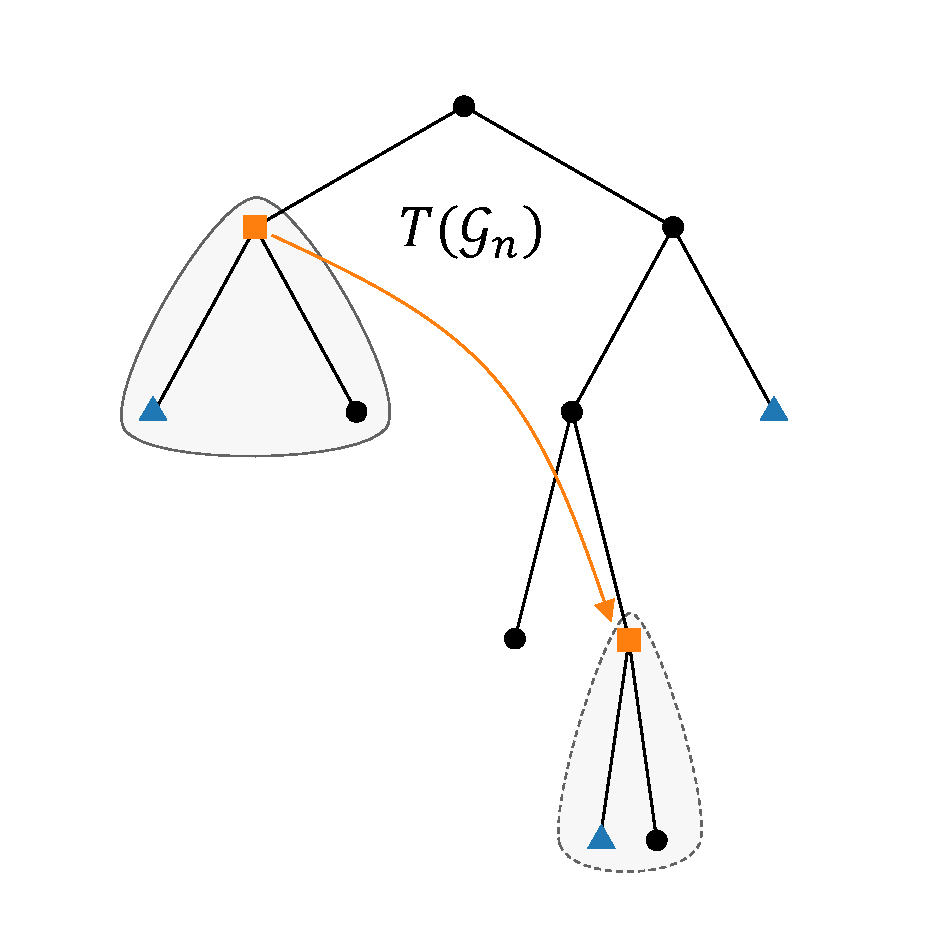
\includegraphics[trim={2.cm 1cm 2.5cm 1cm}, clip, width=0.44\textwidth]{img/gbop/tree_5.pdf}
	\caption{The tree $T(\cG_n)$ obtained by unrolling $\cG_n$. Contrary to $T_n$ shown in \Cref{fig:structures}, the red leaf $a$ is expanded at the same time as the internal red node, which enables to tighten its value bounds $(L_n(a), U_n(a))$ by applying $B_n$.}
	\label{fig:unroll}
\end{figure}
We analyse \GBOPD though the prism of $T(\cG_n)$, which is only used as a theoretical tool. 

We can define the counterpart of the bounds $(\cL_n, \cU_n)$ in the same way as \eqref{eq:opd-bounds} applied to $T(\cG_n)$ rather than $T_n$, except that the depth $d_n$ of $T(\cG_n)$ can now be infinite:
\begin{align}
\label{eq:gbop-t-bounds}
L_n = B_n^{\infty}(0), \qquad U_n = B_n^{\infty}(V_{\max}).
\end{align}
This definition is equivalent to that of \GBOPD in the sense that:
\begin{lemma}[Bound equivalence]
	\label{lem:equivalence}
	For any sequence of action $a\in T(\cG_n)$, we have $L_n(a) = \cL_n(s(a))$ and $U_n(a) = \cU_n(s(a))$.	
\end{lemma}

In $T(\cG_n)$, the unrolling mechanics behave as if any leaf $a$ sharing the same state $s(a)$ as an internal node $a'$ was automatically expanded, and thus had its bound $L_n(a), U_n(a)$ tightened by the Bellman backup $B_n$ to a sub-interval of the trivial bounds $(0, V_{\max})$ that are used in \OPD.

The sampling and recommendation rules of \GBOPD also amount to running those of \OPD on the tree $T(\cG_n)$, except that the sampled sequence $b_n$ and recommended sequence $a_n$ can now have infinite depth since $T(\cG_n)$ itself can be infinite (we say that $a_n$ and $b_n$ are represented by nodes of infinite depth). In the sequel, we analyse how these rules behave on $T(\cG_n)$.

\begin{lemma}[Expansion]
	\begin{leftbar}[lemmabar]
	\label{lem:expansion-bound}
	Any node $a$ of depth $h$ traversed by the optimistic sampling rule of \GBOPD at iteration $n$ belongs to $T_h^\infty(L_n, U_n)$: 
	\begin{equation}
	\label{eq:expansion-regret}
	V^\star-V(a) \leq \gamma^h(U_n(a)-L_n(a)).
	\end{equation}
	
	In particular, if the sampling rule samples an infinite sequence $a\in A^\infty$, it is an optimal sequence, and we write that \eqref{alg:gbop-d} also holds for $a$ with $h=\infty$.
	\end{leftbar}
\end{lemma}


\begin{lemma}[Recommendation]
	\begin{leftbar}[lemmabar]
	\label{lem:recommendation-bound}
	The action $a_n$ recommended by \GBOPD has a simple regret $r_n \leq \frac{\gamma^{d_n}}{1-\gamma}$, where $d_n\in\Real\cup\{\infty\}$ is the maximal depth of expanded nodes in $T(\cG_n)$.
	\end{leftbar}
\end{lemma}
Note that even though $T(\cG_n)$ can be infinite, there is only one node $b_t$ that is selected for expansion at each iteration $t\leq n$.

\subsubsection{Regret guarantee}

In \Cref{thm:regret-bound-U}, we assumed that some bounds $(L,\,U)$ were revealed by an oracle and available from the onset for planning. In \eqref{eq:gbop-t-bounds}, we instead built a \emph{sequence} of bounds $(L_n,U_n)_{n\geq 0}$ \eqref{eq:gbop-t-bounds} that is non-increasing in the sense of inclusion, i.e. $0\leq \dots\leq L_{n-1}\leq L_n\leq V\leq U_n\leq U_{n-1}\leq \dots\leq V_{\max}$.

We can consider the sequence $\kappa_n = \kappa(L_n, U_n)$. It is non-increasing and lower-bounded by $1$, thus converges. Let $\hlgb{\kappa_\infty = \lim_{n\rightarrow\infty} \kappa(L_n, U_n)} \in[1,K]$.

\begin{theorem}
	\begin{leftbar}[theorembar]
	\label{thm:regret-gbop}
	\GBOPD enjoys the following regret bound, with $\hlgb{\kappa_\infty} \leq \hlrb{\kappa}$: 
	\begin{align*}
	r_n = \tilde{\cO}\left(n^{-\log \frac{1}{\gamma}/\hlgb{\log \kappa_\infty}}\right).
	\end{align*}
	\end{leftbar}
\end{theorem}

Intuitively, $\kappa_\infty$ should be much lower than $\kappa$ in problems where trajectories overlap a lot. For instance, it will be the case for problems where two actions cancel each-other out (e.g. moving left or right), or are commutative (e.g. placing pawns on a board game). However, this is merely an intuition. We now show that there exist problem instances in which $\hlgb{\kappa_\infty} < \hlrb{\kappa}$, which is a legitimate concern since their non-existence would make \Cref{thm:regret-gbop} trivial.

\subsubsection{Illustrative example}

We consider a toy MDP $\cM$ shown in \Cref{fig:mdp}. The transitions are described visually while the rewards are defined as follows: let $0\leq r^\star\leq \gamma$, and $ r^- = r^\star - \frac{\gamma}{1-\gamma} S$, $r^+ = r^\star + S$ with $S = r^\star\left(\frac{1}{\gamma} - 1\right).$ Note that the choice ensures that $r^\star, r^-, r^+$ and $S$ are all in $[0, 1]$.

\begin{figure}[htp]
	\centering
	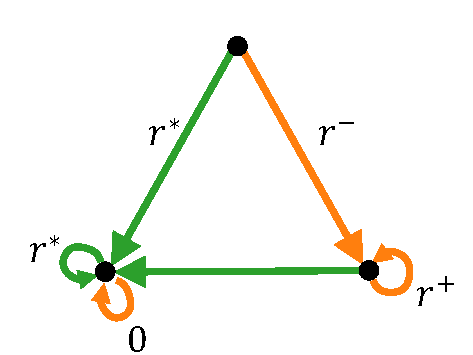
\includegraphics[trim={0.5cm 0.0cm 0.3cm 0.6cm}, clip, width=0.35\textwidth]{img/gbop/mdp.pdf}
	\caption{A toy MDP with three states and $K \geq 2$ actions. We start in the top state. The first action $a_1$ is represented by \textcolor{lightgreen}{green} arrows, and all other actions $a_2, \dots, a_K$ are represented by \textcolor{Orange}{orange} arrows. The rewards are shown next to the transitions.}
	\label{fig:mdp}
\end{figure}

\begin{proposition}[Comparison of branching factors]
	\begin{leftbar}[propositionbar]
	\label{prop:illustrative-example}
	The MDP $\cM$ verifies $\hlrb{\kappa = K-1}$ and $\hlgb{\kappa_\infty = 1}$.
	% :
	% \begin{enumerate}[label=(\roman*)]
	%     \item $\hlrb{\kappa = K-1}$;
	%     \item $\hlgb{\kappa_\infty = 1}$.
	% \end{enumerate}
	\end{leftbar}
\end{proposition}
This result confirms that \Cref{thm:regret-gbop} is non-trivial since we exhibit a problem for which $\hlgb{\kappa_\infty} < \hlrb{\kappa}$ (when $K\geq 3$), and legitimates our attempt to improve planning performances by merging the tree into a graph.


\subsection{Extension to Stochastic Systems}
\label{sec:stochastic}

The approach developed in \Cref{sec:gbopd,sec:analysis} consists in using state similarity to tighten a pair of lower and upper bounds $(L,\,U)$ for the value function $V$. Thus, any planning algorithm that is based on such bounds can benefit from this insight, and any theoretical result based on the validity and rate of convergence of these bounds will be preserved.  

\paragraph{Confidence intervals for rewards.}

When the reward kernel $P\left(r \condbar s,a\right)$ is stochastic, deviation inequalities can be used to design a confidence interval $[\ell_t(s,a), u_t(s,a)]$ over its expected value $\expectedvalue\left[r | s,a\right]$. For instance, the Chernoff-Hoeffding deviation inequality was used to design confidence intervals in \citep{Kocsis06UCT,Bubeck2010open,Kaufmann2017}.
In recent works \citep{Leurent2019practical, MDPGapE2020}, the tighter Kullback-Leibler confidence interval is preferred:
\begin{align*}
u_t(s,a) &\eqdef \max \left\{v : \kl\!\big(\hat{r}_t(s,a),v\big) \leq \frac {\beta^r(n_t(s,a), n)} {n_t(s,a)} \right\},\\
\ell_t(s,a) &\eqdef\min \left\{v : \kl\!\big(\hat{r}_t(s,a),v\big) \leq \frac {\beta^r(n_t(s,a), n)} {n_t(s,a)} \right\},
\end{align*}
where $\hat{r}_t(s,a)$ is the sample mean, $\beta^r$ is an exploration function and $\kl(u,v)$ is the binary Kullback-Leibler divergence between Bernoulli distributions: $\kl(u,v) = u \log \tfrac {u} {v} + (1-u) \log \tfrac {1-u} {1-v}$.

\paragraph{Confidence region for transitions.}

Likewise, when the transition kernel $P\left(s' \condbar s,a\right)$ is stochastic, a confidence set on the probability vector $p(\cdot|s,a)$ can be defined as
$\cC_t(s,a) \eqdef \left\{p\in \Sigma_S :  \KL\!\big(\hp_t(\cdot|s,a),p\big) \leq \frac {\beta^p(n_t(s,a), n)} {n_t(s,a)}\right\}$,
where $\Sigma_S$ is the probability simplex over $S$, $\beta^p$ is an exploration function and $\KL(p,q)= \sum_{s \in S}  p(s) \log \tfrac{ p(s)} {{q}(s)}$ is the Kullback-Leibler divergence between categorical distributions.

\paragraph{Bellman operator with stochasticity.}

In this work, we do not discuss the tuning of $\beta^r$, $\beta^p$, but simply assume that they are chosen such that the rewards and transitions belong to their confidence regions with sufficiently high probability to obtain performance guarantees for the  planning algorithm. For more details on such a choice, refer to \citep[e.g.][]{Leurent2019practical, MDPGapE2020}. We modify the \Cref{def:bellman} of the Bellman operator on graphs as:

\begin{align*}
\cB_t^+(\cU)(s) &= \max_{a\in A} \left[u_t(s,a) + \gamma \max_{p \in \cC_t(s,a)} \sum_{s'} p(s'|s,a) \cU(s')\right], \\
\cB_t^-(\cL)(s) &= \max_{a\in A} \left[\ell_t(s,a) + \gamma \min_{p \in \cC_t(s,a)} \sum_{s'} p(s'|s,a)\cL(s')\right],
\end{align*}
for all $s\in\inte{\cG_n}$, where the maximum and minimum over these Kullback-Leibler confidence regions $\cC_t(s,a)$ can be computed as explained in \citep[Appendix A of][]{Filippi2010optimism}. Under the event that every confidence regions $[\ell_t(s,a), u_t(s,a)]$ and $\cC_t(s,a)$ are valid at time $t$, the \Cref{lem:properties-b-graph} still holds for $\cB_t^-, \cB_t^+$.

\paragraph{Structure of the planning algorithm}

In the deterministic setting, once a transition has been observed, it is known with certainty and doesn't need to be sampled ever again, which is why only external nodes $\ext{\cG_n}$ are sampled in \GBOPD. Conversely, in the stochastic setting the expected reward and transition probabilities must be estimated from samples, which implies that internal nodes $\inte{\cG_n}$ must be sampled as well. Then, it is common to adopt and episodic setting where we sample trajectories of a fixed horizon $H$, tuned depending on the budget $n$. This is the case in  \citep[e.g.][]{Kearns02SS,Kocsis06UCT,Bubeck2010open,Feldman14BRUE,Leurent2019practical,MDPGapE2020}. We also follow this scheme in our proposed \GBOP

\begin{algorithm}[ht]
	\caption{\emph{Graph-Based Optimistic Planning} (\GBOP) algorithm.}
	\label{alg:gbop}
	\DontPrintSemicolon
	\For{trajectory $m$ in $[1, M]$}{
		\For{time $t$ in $[1, H]$}{
			$n \gets (m - 1)H + h$.\;
			Compute the bounds $\cL_n = (\cB_n^-)^{\infty}(0)$ and $\cU_n = (\cB_n^+)^\infty(V_{\max})$.\; 
			$b_t\gets \displaystyle\argmax_{a\in A} r(s_t, a) + \gamma \cU_n(s')$ \Comment*[r]{Optimistic sampling rule}
			Simulate $r_t, s_{t+1} \sim P\left(r, s_{t+1} \condbar s_t, b_t\right)$.\;
			Get or create the node $s_{t+1}$ in $\cG_{n+1}$, and add an occurence of the transition $(s_t,b_t, r_t, s_{t+1})$.
		}
	}
	\Return $\displaystyle\argmax_{a\in A} r(s,a) + \gamma \cL_n(s(a))$. \Comment*[r]{Conservative recommendation rule}
\end{algorithm}

\subsection{Numerical Experiments}
\label{sec:experiments}

To evaluate the practical benefits of our approach, we compare graph-based and tree-based planning algorithms in various problems.

\paragraph{Gridworld domain.}
We consider a grid in which the agent can move in $K=4$ directions. The reward function is $0$ everywhere, except in the vicinity of a goal located at $(10, 10)$, around which the reward decreases quadratically from $1$ to $0$ in a ball of radius $5$. %: $r(x, y) = \max(1 - \frac{1}{5^2}((x-10)^2 + (y-10)^2), 0)$. 
The \Cref{fig:deterministic-gridworld} shows number of times a state is sampled by \OPD and \GBOPD, both run with a budget $n = 5460$ and discount $\gamma=0.95$. In the absence of rewards, \OPD samples sequences of actions uniformly (in a breadth-first search manner), which --because of the dynamics structure-- results in a non-uniform occupancy of the state space $S$, where the trajectories concentrate near the starting state. In contrast, \GBOPD explores uniformly in $S$, sampling each state up to four times (from its four  neighbours), until it finds the goal vicinity and finally samples the goal location indefinitely. We reproduce the experiment in the stochastic setting by adding noise on the transitions with probability $p=10\%$, and comparing \GBOP to \texttt{UCT} as we show in \Cref{fig:stochastic-gridworld}. To quantify these qualitative differences, we define an exploration score: the average distance $d(s_t, s_0)$ of sampled states to the initial state (exploration) minus the distance $d(s_t, s_g)$ to the goal state (exploitation), that we show in \Cref{fig:exploration-score}.

\begin{figure}[ht]
	\centering
	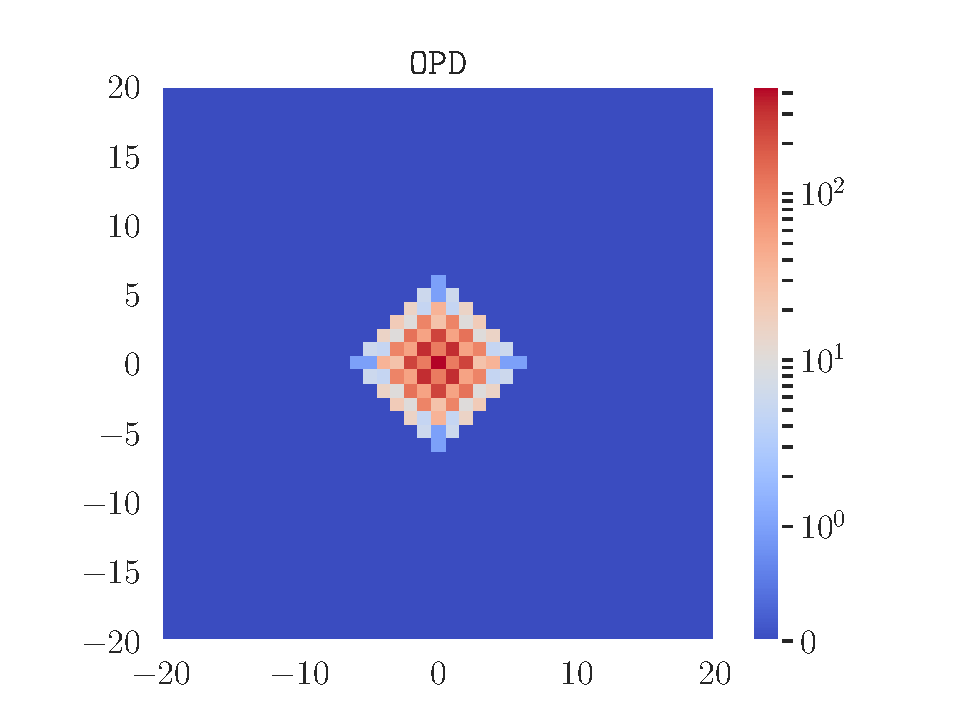
\includegraphics[trim={1.8cm 0.7cm 1.8cm 0.7cm}, clip, width=0.4\linewidth]{img/gbop/occupations_OPD.pdf}
	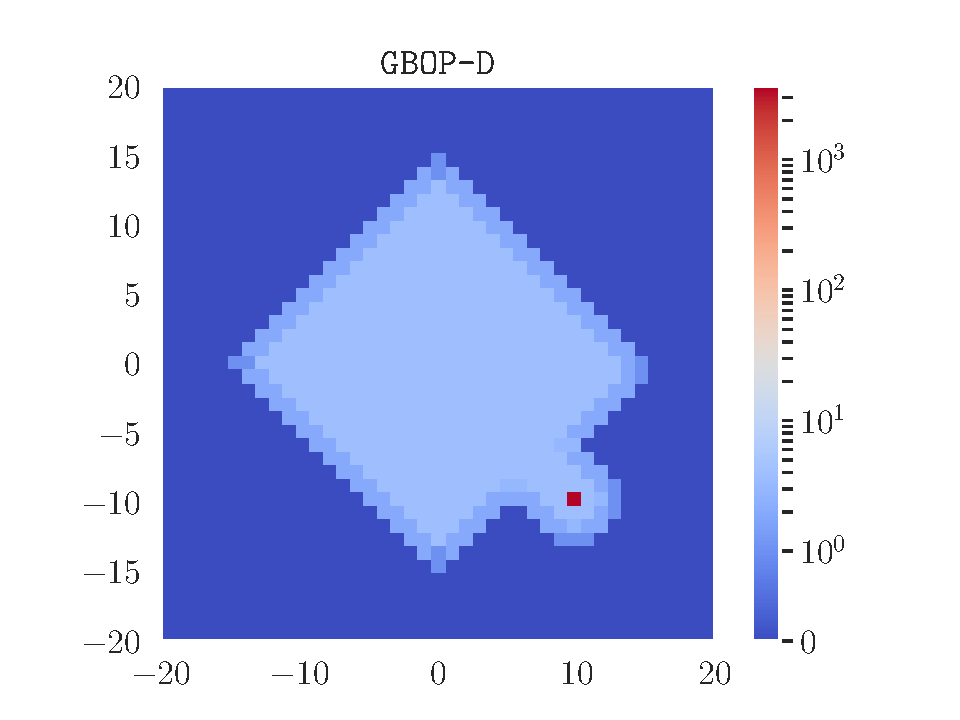
\includegraphics[trim={1.8cm 0.7cm 1.8cm 0.7cm}, clip, width=0.4\linewidth]{img/gbop/occupations_GBOP-D.pdf}
	\caption{State occupancies of two planning algorithms in a deterministic gridworld.}
	\label{fig:deterministic-gridworld}
\end{figure}
\begin{figure}[ht]
	\centering
	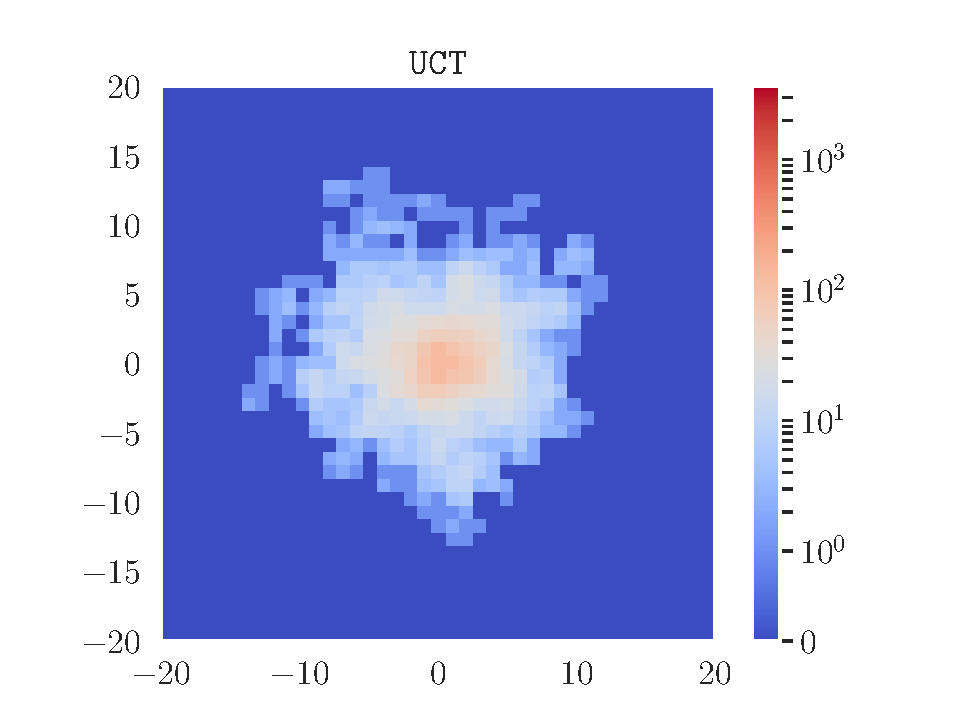
\includegraphics[trim={1.8cm 0.7cm 1.8cm 0.7cm}, clip, width=0.4\linewidth]{img/gbop/occupations_UCT.pdf}
	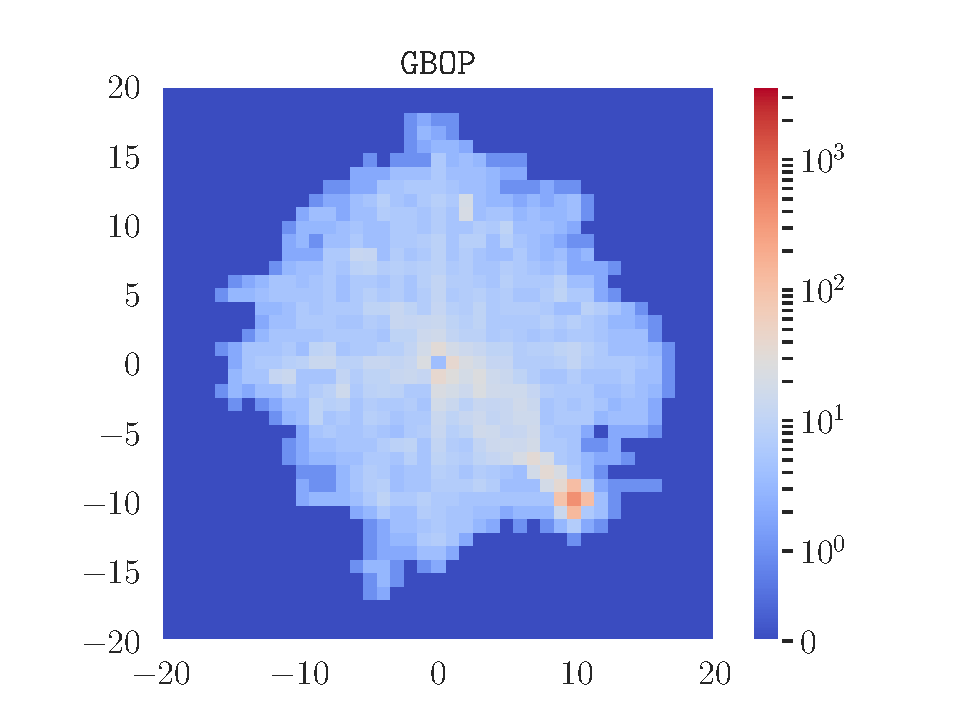
\includegraphics[trim={1.8cm 0.7cm 1.8cm 0.7cm}, clip, width=0.4\linewidth]{img/gbop/occupations_GBOP.pdf}
	\caption{State occupancies of two planning algorithms in a stochastic gridworld.}
	\label{fig:stochastic-gridworld}
\end{figure}

\paragraph{Sailing domain \citep{Vanderbei1996}.}
In a second experiment, a boat is sailing in $K=8$ directions to reach a goal, and suffers a cost (move duration) that depends on the direction of the wind which follows stochastic dynamics. \Cref{fig:sailing} shows the evolution of the simple regret $r_n$ of stochastic planning algorithms with respect to the number $n$ of oracle calls. We show the mean regret and its 95\% confidence interval computed over 500 simulations. The asymptotic log-log slope $\sigma$ provides an empirical measurement of the effective branching factor $\kappa_e = \exp(-\log(1/\gamma)/\sigma)$ for each algorithm. We measure that for $n>10^{3.5}$, $\sigma \approx-0.04$ and $\kappa_e \approx 3.6$ for \texttt{BRUE}, \texttt{KL-OLOP}, \texttt{MDP-GapE}, \texttt{UCT}. In contrast, we measure $\sigma \approx-0.3$ and $\kappa_e \approx 1.2$ for \GBOP, which suggests that our result of \Cref{thm:regret-gbop} might generalize to the stochastic setting. Additional results and experimental details are provided in the Supplementary Material.

\begin{figure}[ht]
	\centering
	\begin{subfigure}[b]{0.49\textwidth}
		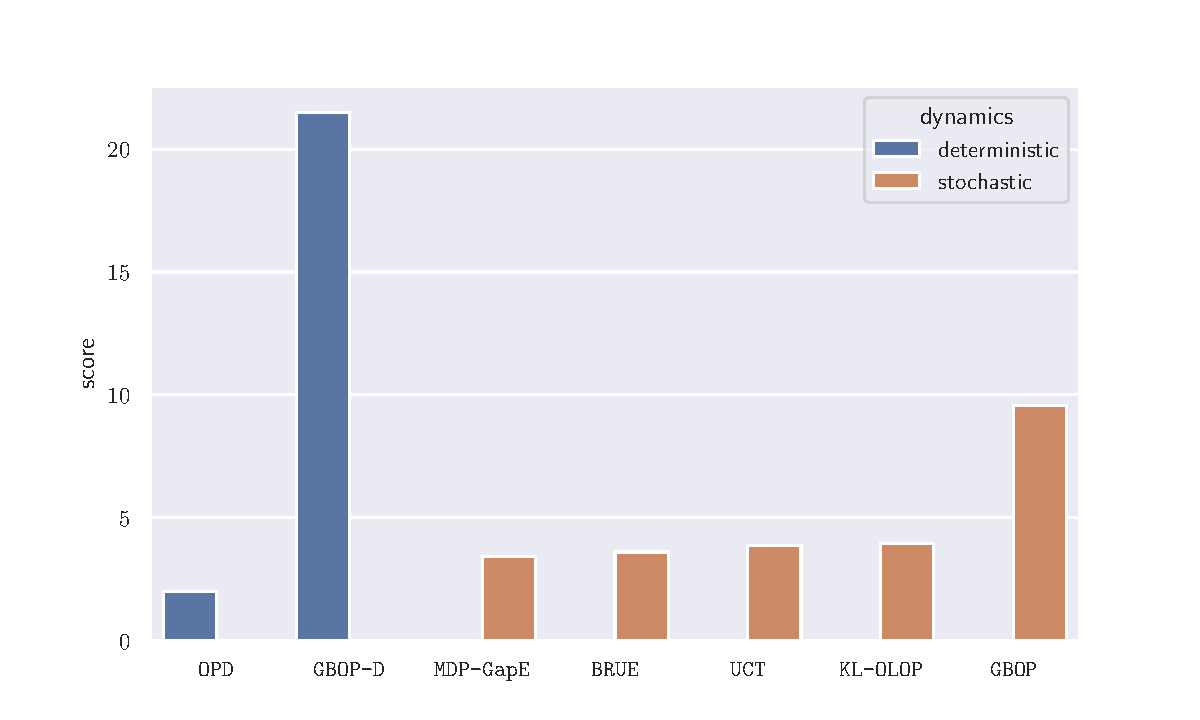
\includegraphics[trim = {1.6cm 0.cm 2cm 1.5cm}, clip, width=\linewidth]{img/gbop/score.pdf}
		\caption{Exploration score in the gridworld domain for several algorithms.}
		\label{fig:exploration-score}
	\end{subfigure}
	\hfill%
	\begin{subfigure}[b]{0.49\textwidth}
		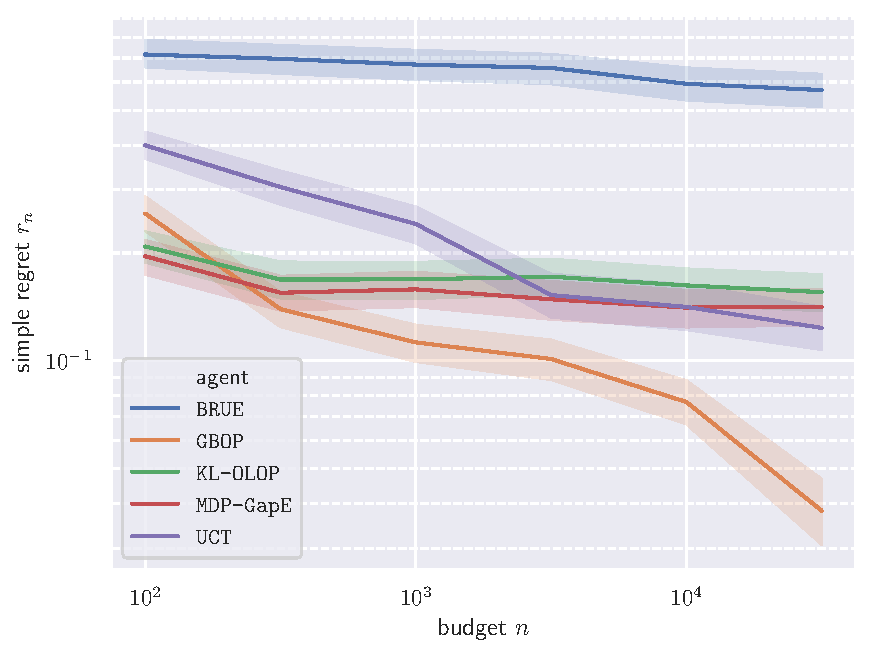
\includegraphics[trim = {0.2cm 0.2cm 0.7cm 0.5cm}, clip, width=\linewidth]{img/gbop/simple_regret.pdf}
		\caption{Mean simple regret $r_n$ in the sailing domain, with its $95\%$ confidence interval.}
		\label{fig:sailing}
	\end{subfigure}
	\caption{Benchmark of planning performances.}
\end{figure}

\subsection*{Conclusion}

We proposed an algorithm that exploits a graph structure to plan in an MDP with a generative model under limited budget $n$. We showed that this graph structure provides a benefit compared to tree structure in the deterministic setting, in the form of an improved regret bound that depends on a smaller problem difficulty. This improvement translates to an enhanced performance in practice, and can be adapted to stochastic problems as we demonstrate experimentally.